%\documentclass[10pt,twocolumn]{article}
\documentclass[11pt]{article}
\usepackage{amsthm}

\usepackage[a4paper,margin=1.8cm,columnsep=0.65cm]{geometry}
\usepackage[T1]{fontenc}

\usepackage{amsthm}

\newtheorem{assumption}{Assumption}
\newtheorem{lemma}{Lemma}
\newtheorem{proposition}{Proposition}
\newtheorem{theorem}{Theorem}
\newtheorem{corollary}{Corollary}

\usepackage[utf8]{inputenc}
\usepackage{lmodern}
\usepackage{microtype}
\usepackage{amsmath,amssymb}
\usepackage{amsthm}
\usepackage{booktabs}
\usepackage{graphicx}
\usepackage{xcolor}
\usepackage{hyperref}
\usepackage[numbers,sort&compress]{natbib}
\usepackage{caption}
\usepackage{enumitem}
\usepackage{amsmath}
\usepackage{placeins}
\hypersetup{colorlinks=true,linkcolor=blue!50!black,citecolor=blue!50!black,
            urlcolor=blue!60!black}
\graphicspath{{figures/}}
\captionsetup{font=small,labelfont=bf}
\setlength{\parindent}{1em}
\setlength{\parskip}{0pt}

% \usepackage{amsthm}
% \newtheorem{assumption}{Assumption}
% \newtheorem{theorem}{Theorem}

\newcommand{\ddg}{\Delta\Delta G}
\newcommand{\model}{ProbJanusDDG}
\newcommand{\kcal}{\mathrm{kcal\,mol^{-1}}}

%\title{\textbf{Conformal Prediction for Protein Stability: Protein-Level Calibration and Sign Reliability}}
\title{Selecting Stabilizing and Destabilizing Protein Mutations with Conformal Prediction}
\author{Guido Barducci\\
\small University of Turin\\
\small \texttt{guido.barducci@unito.it}}
\date{}

\begin{document}
\maketitle

\begin{abstract}
Identifying mutations that increase or decrease protein stability is important for protein engineering and for investigating variants that may affect protein function. However, point predictions alone do not indicate which candidate mutations can be prioritized with greater confidence. To address this limitation,  we introduce ProbJanusDDG, which combines a protein-stability predictor with standard and adaptive conformal prediction intervals.
To calibrate these intervals, a protein-weighted CV+ procedure assigns equal total calibration weight to each protein, accounting for uneven numbers of measured mutations.

For previously uncharacterized mutations, intervals lying entirely above or below zero provide a criterion for selecting candidate stabilizing or destabilizing substitutions, while intervals containing zero leave the direction unresolved. On the external low-homology S669L benchmark, adaptive intervals at the 50\% nominal level assigned directional calls to 34.2\% of mutations, with 94.8\% observed sign accuracy. At the 70\% level, 15.5\% received calls, with 99.0\% sign accuracy.
At the 90\% nominal level, standard and adaptive intervals achieved mutation-level coverage of 91.6\% and 92.5\%, whereas coverage averaged equally across proteins was approximately 87\%. 

Adaptive intervals redistributed width across mutations, with greater widening among predictions with larger observed errors and nearly unchanged mean width.

These results support uncertainty-aware screening of uncharacterized variants: prioritizing candidate stabilizing mutations for protein engineering and candidate destabilizing mutations for investigating stability-related effects on protein function. The method provides a selective criterion for experimental follow-up while distinguishing predictions with a resolved direction from those requiring further evidence.



% Reliable prediction of mutation-induced changes in protein stability (\(\Delta\Delta G\)) requires not only accurate point estimates, but also uncertainty estimates that quantify the reliability of individual predictions. However, calibrated predictive uncertainty remains largely unexplored in protein-stability prediction, where evaluation is further complicated by strongly unbalanced numbers of mutations across proteins.

% Here, we introduce a protein-stability prediction model that combines accurate \(\Delta\Delta G\) prediction with conformal prediction to provide calibrated prediction intervals for individual mutations. The model incorporates a protein-weighted CV+ calibration procedure designed to limit the influence of proteins represented by disproportionately many mutations. To assess the robustness of the conformal calibration strategy, we additionally evaluate it on a deliberately contrasting baseline based on one-hot encoded sequence features. Despite the substantial differences in predictive performance and input representation between the two predictors, conformal calibration produced empirical coverage close to the nominal levels in both cases.

% On the low-homology external S669L test set, the model achieved Pearson \(r=0.53\) and mean absolute error \(0.99\,\mathrm{kcal/mol}\), while the learned relative scale was associated with absolute prediction error (Spearman \(\rho=0.22\)). At 90\% nominal coverage, standard and adaptive protein-weighted intervals covered approximately 92\% and 93\% of mutations, respectively, while coverage averaged equally across proteins was 87\%. Adaptive intervals reduced coverage dispersion across five predicted-uncertainty groups from 4.75 to 3.63 percentage points, with similar mean width (4.96 versus \(5.00\,\mathrm{kcal/mol}\)).
% For a specific mutation, the resulting conformal intervals can be used to determine the highest confidence level at which zero remains excluded, providing a direct practical criterion for assessing whether the predicted effect can still be regarded as stabilizing or destabilizing.

% These results show that the proposed model can provide both accurate protein-stability predictions and empirically calibrated prediction intervals, while mutation-specific scale estimates improve how uncertainty is allocated across individual predictions. More broadly, our results demonstrate how conformal prediction can be integrated into protein-stability models to provide reliable uncertainty estimates and highlight the importance of distinguishing mutation-level from protein-level notions of coverage.
\end{abstract}

\section{Introduction}
The change in folding free energy caused by a mutation, \(\Delta\Delta G\), is a central quantity in protein engineering and in the interpretation of disease-associated variants\cite{mehra2019computational}\cite{meghwanshi2020enzymes}\cite{shi2025recent}. Given its importance, numerous methods have been developed to predict \(\Delta\Delta G\), which can be broadly divided into two main categories: structure-based and sequence-based approaches. Structure-based predictors exploit three-dimensional information about the protein, ranging from local atomic environments to residue- or atom-level interactions modeled through graph and geometric neural networks\cite{li2025generalizable}\cite{li2024prostage}\cite{rossi2025mass}. 
While these approaches can capture detailed structural context, they require an experimentally determined or predicted protein structure. Sequence-based methods, in contrast, operate directly on the amino-acid sequence and span a broad spectrum of complexity, from simple models based on handcrafted or one-hot encoded features to feed-forward neural networks and transformer-based protein language models, which provide contextual residue representations learned from large sequence collections\cite{barducci2026janusddg}\cite{savojardo2025ddgemb}. Consequently, current protein-stability predictors differ substantially in their input information, representations, architectures, and overall model complexity.

Despite this diversity, most $\Delta\Delta G$ predictors still provide only a
point estimate, with no directly interpretable measure of the reliability of
individual predictions\cite{sanavia2020limitations}\cite{qiu2024review}. Previous attempts to address this limitation include
BayeStab, which uses a Bayesian neural network with concrete dropout to estimate
predictive uncertainty and separate aleatoric and epistemic components
\cite{wang2022bayestab}. However, its uncertainty estimates are primarily used
to characterize sources of prediction error and are not calibrated against
prespecified coverage levels. Consequently, they do not directly provide a
prediction interval with an interpretable reliability level for an individual
mutation. 
%This limits their practical use in settings where the uncertainty associated with a specific prediction is itself relevant, for example when deciding whether the predicted effect can be confidently classified as stabilizing or destabilizing. 
%Therefore, these uncertainty estimates do not directly quantify the confidence associated with an individual prediction in terms of a calibrated coverage level, which limits their interpretability for mutation-specific assessment.

A complementary approach was proposed by Sapozhnikov et al.~\cite{sapozhnikov2023statistical}, who modeled the absolute error of FoldX predictions using linear regression and constructed mutation-specific prediction intervals. Although these intervals support uncertainty-aware interpretation of stability effects, their validity relies on the assumptions underlying the regression model, rather than distribution-free conformal calibration. Moreover, folding-stability validation involved only ten proteins, and aggregate coverage was calculated by pooling mutations, giving greater influence to proteins with more measurements. Despite approximately 95\% aggregate coverage, coverage for individual proteins fell as low as 79\%. These results highlight the importance of distinguishing mutation-level coverage from coverage averaged equally across proteins when assessing generalization to previously unseen proteins.

Moreover, the required level of information depends on the application: in some settings an accurate estimate of the magnitude of \(\Delta\Delta G\) is important, whereas in others it may be sufficient to determine, with quantified uncertainty, whether a mutation is expected to stabilize or destabilize the protein \cite{pancotti2022predicting}. Conformal prediction intervals provide a natural way to address both settings, by quantifying uncertainty around the predicted magnitude and by distinguishing predictions whose plausible values lie entirely on one side of zero from those for which the direction of the effect remains uncertain. These considerations motivate uncertainty-quantification strategies that are both reliable and largely independent of the underlying predictive architecture\cite{romano2019conformalized}\cite{zhou2025conformal}\cite{angelopoulos2024theoretical}.

In this paper, we introduce a new predictor of mutation-induced changes in protein stability (figure~\ref{fig:probjanus}a) that provides both point estimates of \(\Delta\Delta G\) and calibrated prediction intervals for individual mutations. The model is designed to produce an exactly antisymmetric mean prediction together with an exactly symmetric mutation-specific uncertainty estimate. This uncertainty estimate is used to construct both standard and adaptive conformal prediction intervals, with adaptive widths modulated according to the predicted relative error scale. Calibration is performed using held-out residuals and predictions from the corresponding fold model, while equal total weight is assigned to each WT protein to reduce the influence of proteins represented by disproportionately many mutations. Point predictions are obtained as the median across five fold models. The overall prediction and calibration procedure, including ensemble aggregation across fold models, is illustrated in Figure~~\ref{fig:probjanus}b.

Although developed here as part of our predictor, the conformal calibration strategy is model-agnostic and can, in principle, be applied to predictors with different architectures and input representations. To illustrate the model-agnostic nature of the conformal calibration procedure, we additionally apply the same approach to a deliberately simple model based on one-hot encoded sequence features. This provides a contrasting test case showing the adaptability of the concept to a substantially different model with different performance, while using the same calibration strategy.


\section{Materials and methods}

\subsection{Task and sign convention}

For a wild-type protein sequence $x_w$ and a mutant sequence $x_m$, the model predicts
$\ddg(x_w,x_m)$. We use the convention that positive $\ddg$ indicates stabilization and negative
$\ddg$ indicates destabilization\cite{capriotti2004neural}. Reversing a mutation changes the sign of the physical target, since Gibbs free energy is a state function and the corresponding free-energy difference depends only on the initial and final states:
\begin{equation}
\ddg(x_m,x_w)=-\ddg(x_w,x_m).
\end{equation}

\subsection{Datasets and splitting}
The training set used in this work is S2450, a refined version of the widely used S2648 collection\cite{savojardo2025ddgemb}. S2648 contains 2,648 experimentally characterized single-amino-acid substitutions across 131 proteins, with \(\Delta\Delta G\) values originally obtained from the ProTherm database\cite{dehouck2011popmusic}. In the construction of S2450, sequence similarity with the S669 benchmark was re-evaluated using full-length UniProt sequences rather than PDB sequences. Proteins from S2648 sharing more than 25\% sequence identity with any protein in S669 were removed, resulting in the exclusion of 18 proteins and 198 mutations. The final S2450 dataset therefore contains 2,450 single-amino-acid substitutions from 115 protein sequences and provides a training set with reduced sequence overlap with the external benchmark.

For model development, we retained the five protein-disjoint benchmark folds associated with S2450. These folds were constructed using a 25\% sequence-identity threshold to minimize sequence redundancy between training and validation subsets and contain 417, 772, 573, 511, and 177 mutations, respectively. Such protein-level separation is particularly important for \(\Delta\Delta G\) prediction, since multiple mutations are often available for the same protein and random mutation-level splitting could therefore lead to overly optimistic performance estimates\cite{barducci2026janusddg}.

External evaluation was performed on S669L and S461L, the full-length-sequence versions of two established blind benchmarks. S669\cite{pancotti2022predicting} was specifically designed to assess generalization to proteins with low similarity to commonly used training collections, with sequence identity below 25\% relative to datasets such as S2648 and VariBench\cite{nair2013v}. The original benchmark contains both direct and reverse variants across 95 protein chains, with experimentally determined \(\Delta\Delta G\) values collected from ThermoMutDB and manually verified. In the present work, we use S669L, containing 669 mutations from 87 proteins after mapping to the corresponding full-length sequences.
S461 is a curated benchmark derived from S669 and was introduced to remove possible problematic proteins~\cite{hernandez2023predicting}.
%to address inaccuracies in the original dataset and to remove variants potentially associated with natural protein function, including mutations located at oligomeric interfaces. 
It contains 461 single-site mutations with one experimental \(\Delta\Delta G\) measurement per variant. We use its full-length-sequence version, S461L, comprising 461 mutations from 46 proteins. Together, S669L and S461L provide complementary external tests of model generalization under low sequence similarity to the training data.

\subsection{Model Architecture}

In this section, we describe the architecture of the main model used in this study, illustrated in Figure~\ref{fig:probjanus}a.


\subsubsection{Frozen protein language-model representations}

Wild-type and mutant sequences were embedded independently using the 650-million-parameter ESM-2 model~\citep{lin2023evolutionary}. For each residue, ESM-2 provides a 1,280-dimensional contextual embedding. The language-model parameters were kept frozen throughout training, so ESM-2 was used only as a fixed feature extractor for the downstream $\Delta\Delta G$ predictor.


\subsubsection{Bidirectional probabilistic architecture}

The trainable network is based on the directional design of JanusDDG~\citep{barducci2026janusddg}, with modifications to the output layer to support joint prediction of \(\Delta\Delta G\) and mutation-specific uncertainty. We deliberately retain this established backbone rather than
introducing an additional sequence-processing architecture, allowing the present
work to focus on the incorporation of mutation-specific uncertainty and
conformal calibration. The original architecture is therefore adapted to produce
both an antisymmetric $\Delta\Delta G$ estimate and a symmetric uncertainty
estimate, which is subsequently used to construct calibrated prediction
intervals. A detailed description of the underlying sequence-processing
architecture is provided in the original JanusDDG study.

In contrast to JanusDDG, which directly predicts a single \(\Delta\Delta G\) value, our model is designed to predict a probability distribution over \(\Delta\Delta G\). Specifically, it employs two separate linear output heads to jointly estimate the parameters of a Gaussian distribution: the mean (\(m\)) and an unconstrained scale parameter (\(s\)). The predicted mean \(m\) is the directional central estimate, subsequently antisymmetrized within each fold model and aggregated across models. The scale parameter \(s\) is transformed through a softplus function to ensure positivity, yielding the standard deviation of the predicted Gaussian distribution: \begin{equation}
    \sigma = \operatorname{softplus}(s) + \epsilon.
\end{equation}

Thus, the model outputs both a point prediction, through \(m\), and an associated estimate of predictive uncertainty, through \(\sigma\).


At inference, the same trunk is evaluated in both the direct and inverse directions. If $(m_{w\to m},s_{w\to m})$ and
$(m_{m\to w},s_{m\to w})$ denote the corresponding outputs, the delivered prediction is:
\begin{align}
\mu(x_w,x_m) &= \frac{m_{w\to m}-m_{m\to w}}{2}, \\
\sigma(x_w,x_m) &= \operatorname{softplus}\!\left(\frac{s_{w\to m}+s_{m\to w}}{2}\right)+\epsilon,
\end{align}
with $\epsilon=10^{-3}$. Consequently,
$\mu(x_m,x_w)=-\mu(x_w,x_m)$ and
$\sigma(x_m,x_w)=\sigma(x_w,x_m)$ exactly.

\begin{figure*}
    \centering
    \IfFileExists{figures/probjanus.png}{%
      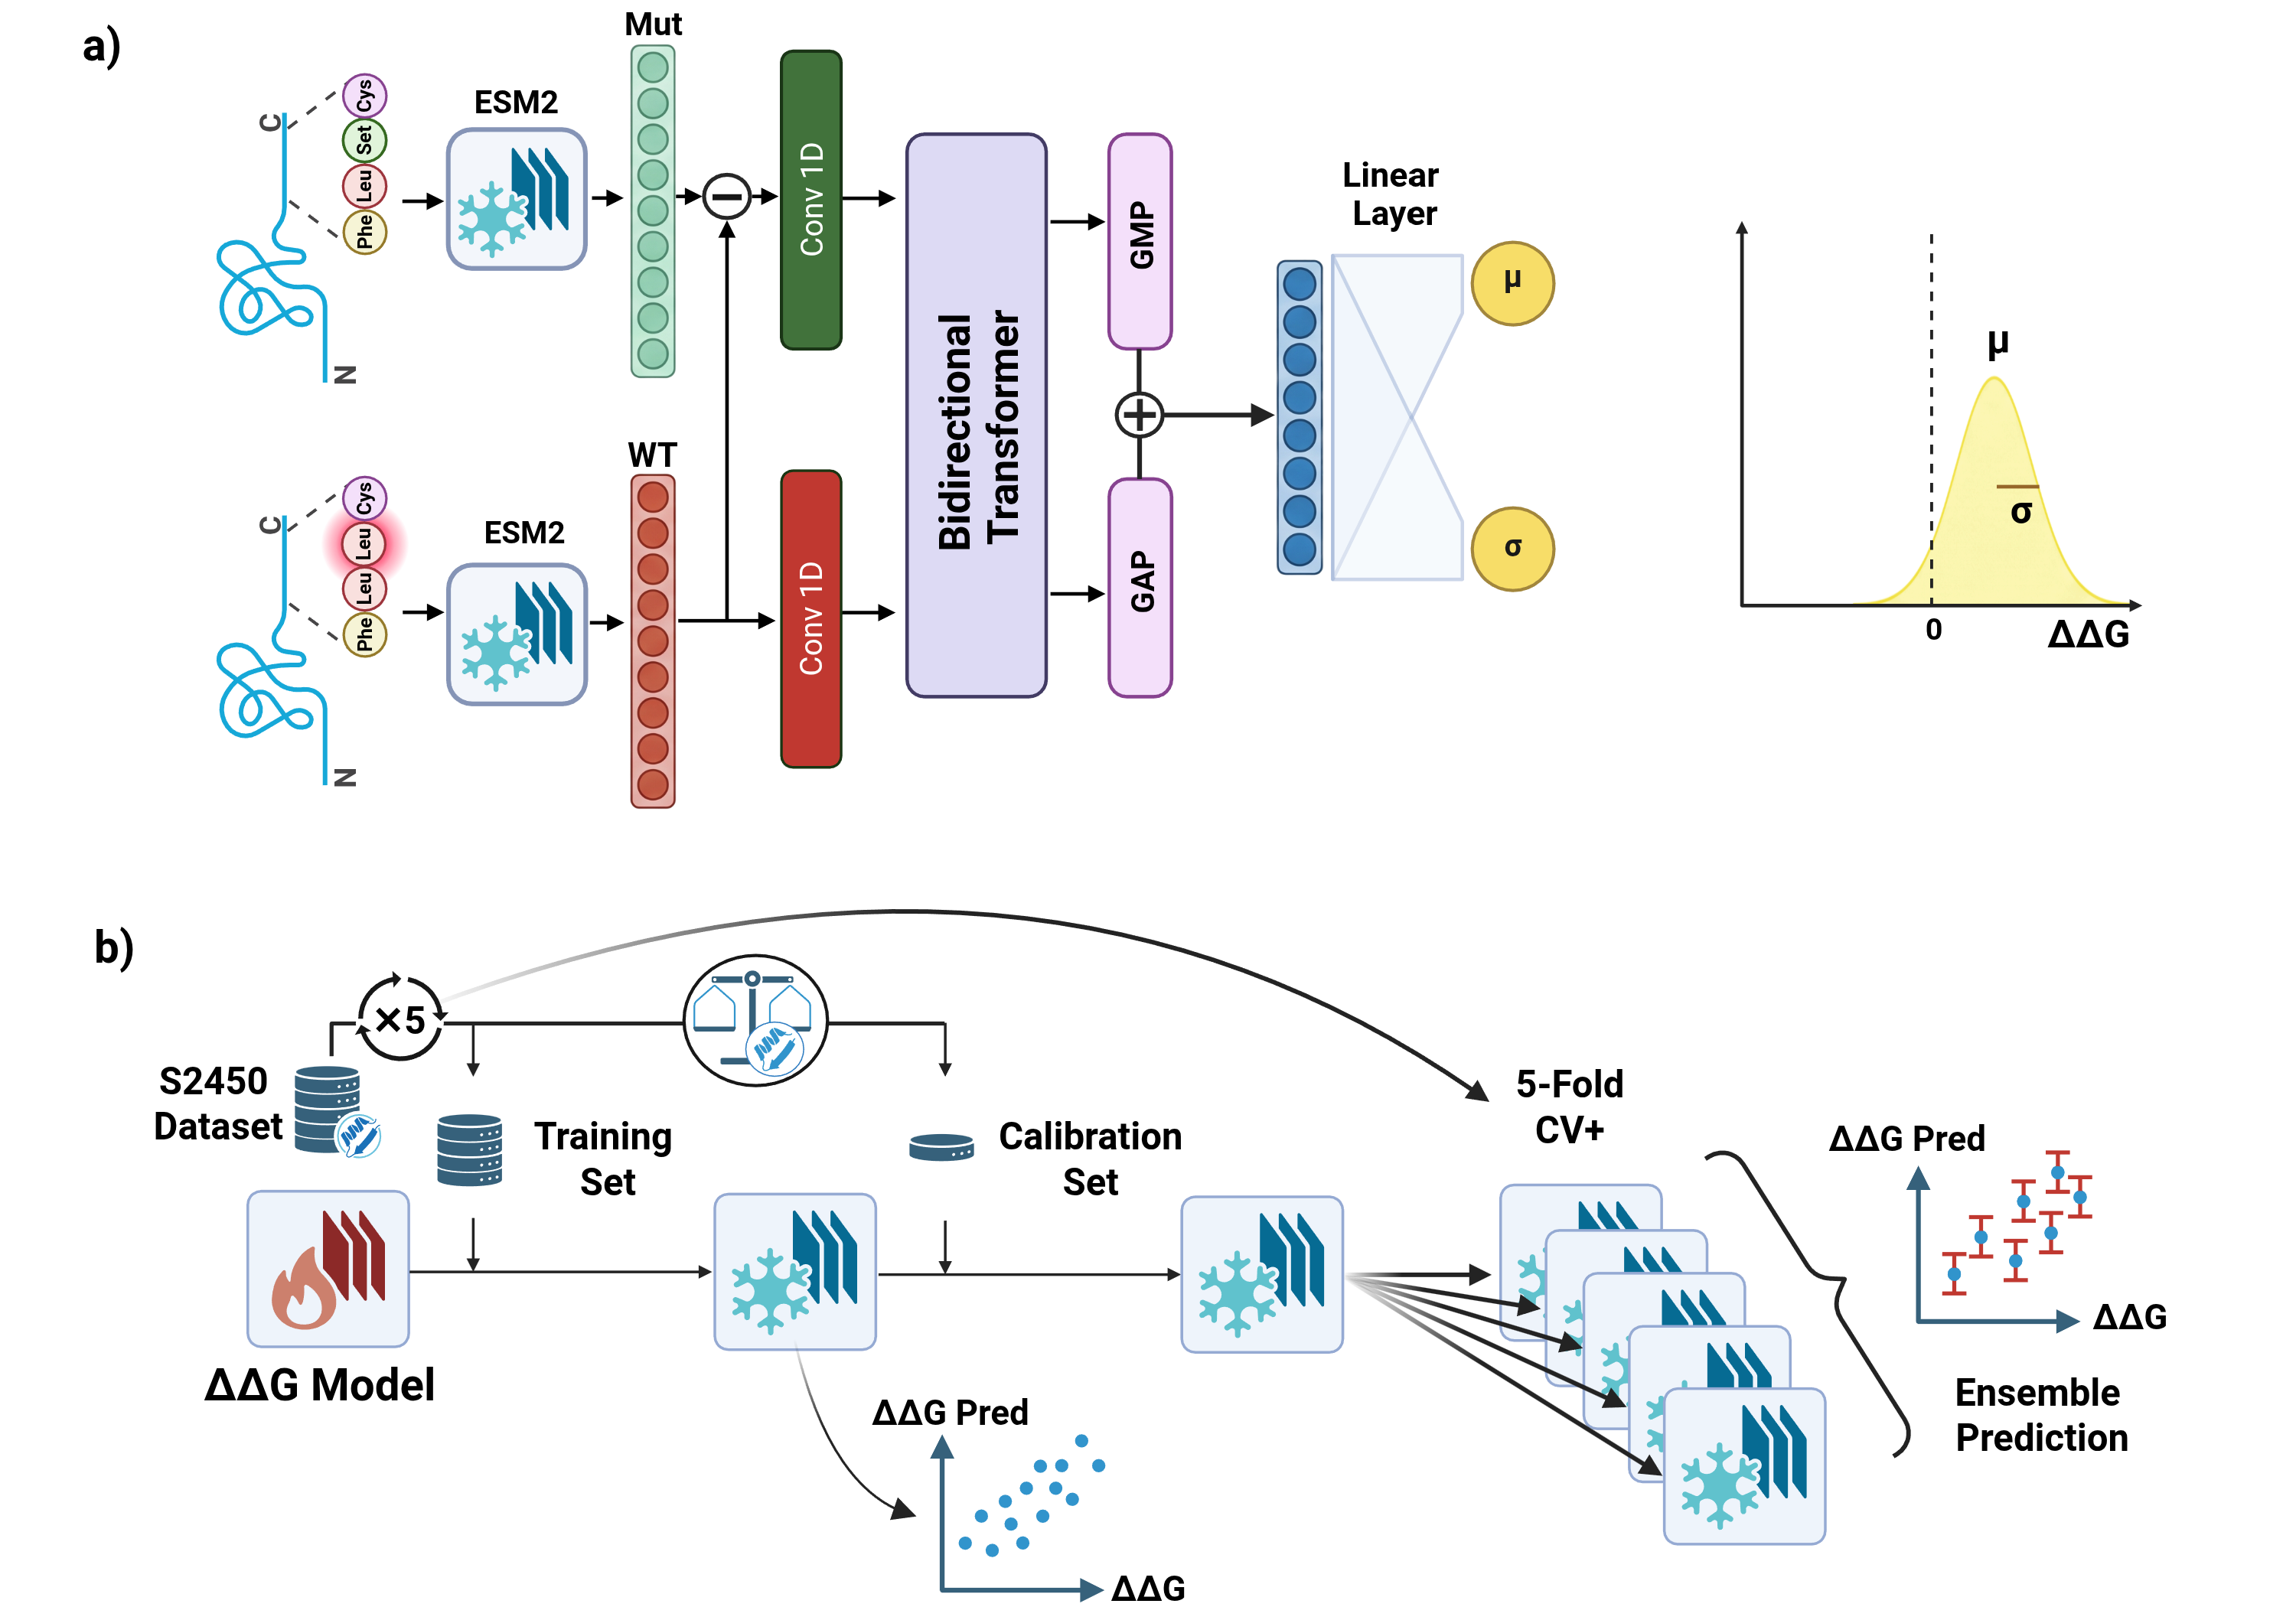
\includegraphics[width=1\linewidth]{figures/overview_probjanus.png}%
    }{%
      \fbox{\parbox[c][2cm][c]{0.75\linewidth}{\centering
      Architecture illustration pending.\\
      Missing file: \texttt{figures/probjanus.png}}}%
    }
    \caption{Schematic overview of ProbJanusDDG and the conformal calibration procedure. (a) Architecture of ProbJanusDDG, which jointly produces a central \(\Delta\Delta G\) prediction and a mutation-specific uncertainty estimate. (b) CV+ calibration pipeline used to combine fold-specific predictions and calibration residuals into standard and adaptive prediction intervals with empirically controlled coverage.
}
    \label{fig:probjanus}
\end{figure*}



\subsection{Directional training with reverse augmentation}

Within each fit, the network is optimized on the selected training mutations and their reverses, obtained by augmenting each observed mutation $(x_w,x_m,y)$ with its reverse $(x_m,x_w,-y)$. During training, the loss is applied directly to the single directional prediction produced for each sample; antisymmetrization is applied only at inference time.

Reverse augmentation encourages the directional predictor to learn the expected antisymmetric behavior of $\Delta\Delta G$. To illustrate this, any directional prediction $f$ can be decomposed into an antisymmetric component $f_A$ and a symmetric component $f_S$, such that $f=f_A+f_S$, where:

\begin{equation}
    f_A(x_w,x_m)=\frac{f(x_w,x_m)-f(x_m,x_w)}{2},
\end{equation}
\begin{equation}
f_S(x_w,x_m)=\frac{f(x_w,x_m)+f(x_m,x_w)}{2}.
\end{equation}

Considering the contributions of a mutation and its reverse to the overall squared-error objective gives:
\begin{equation}
    (y-f(x_w,x_m))^2+(-y-f(x_m,x_w))^2 =
    2(y-f_A)^2+2f_S^2.
\end{equation}
This identity illustrates the effect for an unweighted squared-error objective. The same mechanism also applies to the mean prediction in our Gaussian training objective, while the learned directional scales introduce additional terms in the loss. 

At inference time, antisymmetry is enforced explicitly by evaluating the network in both directions and combining the two predictions as:
\begin{equation}
    \hat{f}(x_w,x_m) =
    \frac{f(x_w,x_m)-f(x_m,x_w)}{2}.
\end{equation}
This operation extracts the antisymmetric component of the directional predictor and guarantees that reversing a mutation changes the sign of the predicted $\Delta\Delta G$.
In contrast, if the loss is computed on an explicitly antisymmetrized prediction,

\begin{equation}
f_{\mathrm{AS}}(x_w,x_m)=\frac{f(x_w,x_m)-f(x_m,x_w)}{2},    
\end{equation}

the symmetric component is removed by construction before the loss is evaluated. Therefore, no separate ($f_S^2$) penalty arises: the optimization acts only on the antisymmetric prediction ($f_{\mathrm{AS}}$), which satisfies ($f_{\mathrm{AS}}(x_w,x_m)=-f_{\mathrm{AS}}(x_m,x_w)$) exactly.


The predictive mean and uncertainty are trained using the heteroscedastic Gaussian negative log-likelihood:
\begin{equation}
    \mathcal{L}(y,\mu,\sigma) =
    \log\sigma+
    \frac{1}{2}\left(\frac{y-\mu}{\sigma}\right)^2,
\end{equation}
where the training outputs are directional and $\sigma=\operatorname{softplus}(s)+\epsilon$. This is the $\beta=0$ member of the $\beta$-NLL family \citep{seitzer2022pitfalls}. Optimization used Adam with a learning rate of $10^{-4}$, a batch size of 6 and a maximum of 300 epochs during cross-validation.

\subsection{Nested epoch selection and four-fold refitting}

Let $\mathcal V_0,\ldots,\mathcal V_4$ denote the five fixed protein-disjoint folds.
For outer fold $k$, the internal validation fold is \begin{math}
    v(k)=(k+1)\bmod 5
\end{math}.
A newly initialized model is trained for 300 epochs on the other three folds, excluding both
$\mathcal V_k$ and $\mathcal V_{v(k)}$. The complete internal validation fold is used
for epoch selection. If $\mathcal P_v$
is its set of WT proteins and $n_{p,v}$ its number of mutations from protein $p$, the validation metric used for epoch selection is:
\begin{equation}
\mathrm{MSE}_{\rm prot}^{(k)}(e)=\frac{1}{|\mathcal P_v|}
\sum_{p\in\mathcal P_v}\frac{1}{n_{p,v}}
\sum_{i\in p\cap\mathcal V_v}(y_i-\mu_{k,e}(x_i))^2.
\end{equation}
The prediction $\mu_{k,e}$ uses the antisymmetric inference rule. Each protein contributes
equally to epoch selection, whereas the Gaussian training loss assigns equal weight to
individual directional examples. This strategy keeps model optimization likelihood-based, while using a protein-balanced validation metric for epoch selection. By giving each protein equal weight, it reduces the influence of proteins represented by many mutations, although estimates for proteins with only a few variants may be less stable.

The selected epoch is the raw minimum over 1--300, with the earliest epoch resolving ties;
no smoothing or patience is used. A new model is then initialized and fitted on all four
folds other than $\mathcal V_k$ for that number of epochs, without validation.
The number of epochs, rather than the number of optimizer steps, is transferred to the refit.
Only this refitted model supplies the residuals on $\mathcal V_k$ and its external predictions.
This construction ensures that, for each outer fold, calibration residuals are obtained from a model that has never used that fold during either training or model selection, thereby preserving a strict separation between model fitting and calibration.
The five fitted models are retained; no full-S2450 final model is trained.

% \begin{table}[t]
% \centering
% \caption{Inner selection and refit epochs. The inner fit excludes both listed folds;
% the refit excludes only the outer fold.}
% \label{tab:epochs}
% \begin{tabular}{rrr}
% \toprule
% Outer fold & Inner validation fold & Refit epochs\\
% \midrule
% 0 & 1 & 57\\
% 1 & 2 & 232\\
% 2 & 3 & 126\\
% 3 & 4 & 283\\
% 4 & 0 & 105\\
% \bottomrule
% \end{tabular}
% \end{table}


\subsection{Protein-weighted empirical CV+ intervals}

In this section, we describe how prediction intervals are constructed from the
cross-validated model predictions and calibration residuals using a
protein-weighted empirical CV+ procedure.

For mutation $i$ in outer fold $k(i)$, define:
\begin{equation}
r_i=\frac{|y_i-\mu_{k(i)}(x_i)|}{\sigma_{k(i)}(x_i)}.
\end{equation}
Each original mutation contributes once; reverse-augmentation duplicates are not calibration
observations. For a new input $x$, the adaptive candidates are:
\begin{align}
\ell_i(x)&=\mu_{k(i)}(x)-r_i\sigma_{k(i)}(x),\\
u_i(x)&=\mu_{k(i)}(x)+r_i\sigma_{k(i)}(x).
\end{align}
The standard candidates replace $r_i\sigma_{k(i)}(x)$ with $|y_i-\mu_{k(i)}(x_i)|$.
The residual and the external prediction always use the same checkpoint. Multiplying every
scale of a given model by the same positive constant cancels in its ratio of external to OOF
scale, so no training-median scale normalization is needed.

If the calibration data contain $P$ WT proteins and protein $p$ has $n_p$ mutations,
observation $i$ receives weight:
\begin{equation}
w_i=\frac{1}{P n_{p(i)}},\qquad \sum_iw_i=1.
\end{equation}
For candidate values $z_i$, let
\begin{equation}
Q^w_t(z)=\inf\left\{z:\sum_i w_i\mathbf 1\{z_i\leq z\}\geq t\right\}.
\end{equation}
Our reported interval is:
\begin{equation}
  \begin{split}
    C_{1-\alpha}(x)=
    [L_x(\alpha)=Q^w_{\alpha}(\ell(x)),\\ U_x(\alpha)=Q^w_{1-\alpha}(u(x))].
  \end{split}
\end{equation}
We refer to $1-\alpha$ as the nominal level of
this empirical construction, not as a proven lower bound on its coverage.

Supplementary section~\ref{sec:protein-balanced-cvplus} provides finite-sample
coverage bounds for this protein-balanced construction under aligned
hierarchical sampling and data-independent protein-level fold allocation.
For the empirical quantile rule used here, marginal coverage is bounded
below by $1-2\alpha-\varepsilon_{P,K}(\alpha)$, where $P$ is the number
of calibration proteins and the finite-sample correction is specified
in the appendix. Under the additional assumptions of balanced folds
and a symmetric fitting procedure, this correction is at most
$2/\sqrt{P}$, yielding an asymptotic lower bound of $1-2\alpha$.
These assumptions are not established by the present sequence-based
partitioning and external benchmark curation; coverage under the
experimental protocol is therefore evaluated empirically.



The reported point prediction is
\begin{equation}
\widehat\mu(x)=\operatorname{median}_{k=0,\ldots,4}\mu_k(x).
\end{equation}
It is exactly antisymmetric because it is the median of five antisymmetric predictions.
The interval endpoints are computed from candidates, not by centering a pooled residual
quantile on this median. Consequently, standard CV+ widths are not exactly constant and
neither interval rule is required to be symmetric around $\widehat\mu$.
%Allora qui non so mettiamo teoria che mediana è dentro l'intervallo e la copertura sarebbe 1 - 2 alpha

\subsection{Assumptions and scope of validity}

The proposed calibration framework reflects the hierarchical structure of the data, in which multiple mutations are observed for each protein and proteins contribute unequal numbers of measurements. Its interpretation therefore depends on the target sampling population, the separation between model fitting and calibration, and the transferability of the learned predictive scale to unseen proteins.

\paragraph{Protein-balanced target.}
Calibration assigns the same total weight to each protein, irrespective of the number of observed mutations. This corresponds to a two-stage target population in which a protein is sampled first and a mutation is then sampled from that protein. Weighting mutations from protein \(g\) proportionally to \(1/n_g\) prevents densely sampled proteins from dominating the calibration distribution and shifts the target from mutation-level to protein-balanced performance.

We treat the full wild-type sequence as the operational protein-level cluster. The intended interpretation is that calibration proteins are representative of the population of proteins encountered at deployment, with mutations sampled according to comparable within-protein mechanisms. The weighting corrects unequal representation across observed proteins, but is not intended to correct arbitrary selection bias or distribution shift.

\paragraph{Out-of-fold separation.}
All calibration scores are obtained from models that exclude the corresponding outer-fold protein. The same fold-specific model is then used to generate the prediction-time candidate associated with that score, preserving the CV+ score--prediction pairing. Model selection is performed within the training portion of each outer split, and the held-out protein is therefore excluded from both parameter estimation and epoch selection.

Outer-fold models are trained on overlapping subsets of the data, so the resulting scores are not mutually independent. This dependence is intrinsic to cross-validation and does not alter the fact that each score is computed out of fold.

\paragraph{Learned predictive scale.}
Calibration uses the normalized score

$$
S_i
=
\frac{
\left|Y_i-\widehat f(X_i)\right|
}{
\widehat\sigma(X_i)
},
\qquad
\widehat\sigma(X_i)>0.
$$

The same prediction and scale functions are used for out-of-fold observations and new inputs. No Gaussian residual assumption is required: \(\widehat\sigma\) acts as a learned local scaling factor that allows prediction intervals to adapt to heterogeneous prediction difficulty.

Useful adaptivity requires the relationship between predicted scale and realized error to transfer to unseen proteins. The resulting intervals should therefore be interpreted as prediction intervals for future measured \(\Delta\Delta G\) values, including measurement variability represented in the training data.

\paragraph{Coverage interpretation.}
The method retains the model-specific construction of CV+ while replacing mutation-uniform aggregation with protein-balanced weighted quantiles. Weighted conformal procedures can retain finite-sample guarantees when the weighting scheme is matched to the target sampling distribution; our weights,

$$
w_i\propto\frac{1}{n_{g(i)}},
$$

define a protein-balanced empirical target.
We therefore evaluate calibration primarily through empirical coverage on unseen proteins, together with interval width and scale-calibration diagnostics. The method is designed to provide calibrated uncertainty at the protein-population level; it is not intended to guarantee identical coverage for every individual protein, mutation, predicted scale, or \(\Delta\Delta G\) subgroup.


\subsection{Evaluation}


\label{sec:evaluation}

Evaluation was performed separately on S669L and S461L using the five fitted models and the calibration residuals obtained from S2450. External observations were used exclusively for evaluation. Because S461L is a curated subset overlapping S669L, its results were interpreted as an assessment under a different benchmark composition rather than an independent replication. Point-prediction performance was assessed using Pearson and Spearman correlations, mean absolute error (MAE), and mean squared error (MSE), calculated for the median ensemble prediction with equal weight assigned to each test mutation.

Prediction intervals were evaluated through empirical coverage, width, and interval score. Standard and adaptive CV+ used the same fitted models, out-of-fold observations, and equal-protein calibration weights, allowing their comparison to isolate the effect of residual normalization by the learned scale. For a test set containing $N$ mutations from $P_{\mathrm{test}}$ distinct full-length WT sequences, we calculated both mutation-level and protein-averaged coverage:
\begin{align}
\widehat{c}_{\mathrm{mut}}(\alpha)
&=
\frac{1}{N}
\sum_{i=1}^{N}
\mathbf{1}\{y_i \in C_{1-\alpha}(x_i)\},
\\
\widehat{c}_{\mathrm{prot}}(\alpha)
&=
\frac{1}{P_{\mathrm{test}}}
\sum_{p=1}^{P_{\mathrm{test}}}
\frac{1}{n_{p,\mathrm{test}}}
\sum_{i\in p}
\mathbf{1}\{y_i \in C_{1-\alpha}(x_i)\}.
\end{align}
The latter gives each protein equal influence and is aligned with the protein-balanced calibration target. Coverage curves were evaluated at integer nominal levels from 51\% to 99\%, and calibration discrepancy was summarized by the mean absolute difference between mutation-level coverage and the nominal level across this grid.

Detailed interval comparisons were performed at the 90\% nominal level. We reported the mean full interval width, $u_i-\ell_i$, and the mean interval score,
\begin{equation}
\mathrm{IS}_{\alpha}(\ell,u;y)
=
(u-\ell)
+
\frac{2}{\alpha}(\ell-y)_{+}
+
\frac{2}{\alpha}(y-u)_{+},
\end{equation}
where $(a)_{+}=\max(a,0)$. Lower scores indicate a better balance between interval width and penalties for uncovered observations. Width and interval score were averaged with equal weight per mutation and were used only for evaluation, not model selection.

To assess the information carried by the learned scale, each model's scale for a test mutation was converted to its percentile within that model's held-out calibration-scale distribution, using midranks for ties. The mean of the five percentiles defined an uncertainty rank, whose association with absolute median-prediction error was measured using Spearman correlation. Fixed percentile boundaries at 0.2, 0.4, 0.6, and 0.8 defined five uncertainty groups, which need not contain equal numbers of test mutations. Coverage heterogeneity was summarized by the population standard deviation of the five mutation-level group coverages, expressed in percentage points.

The redistribution of interval width was examined through paired adaptive-minus-standard width differences, including summaries within quintiles of observed absolute prediction error. These error-based groups were used exclusively for post-hoc interpretation. All mutations whose coverage status changed between the two interval definitions were displayed as illustrative cases.

The practical utility of adaptive intervals was assessed through directional calls at integer nominal levels from 50\% to 95\%. Under our sign convention, an interval lying strictly above zero indicated a stabilizing effect, whereas an interval lying strictly below zero indicated a destabilizing effect; intervals containing or touching zero yielded no directional call. At each level, we reported the proportion of all test mutations receiving a call, the observed sign accuracy among called mutations, and the proportion of distinct WT proteins with at least one call. Sign accuracy assigned equal weight to each called mutation; observed targets equal to zero counted as incorrect calls, and accuracy was undefined when no calls were made. These empirical selective accuracies were distinguished from nominal interval coverage.

Where reported, 95\% uncertainty intervals were obtained from 4,000 paired protein-cluster bootstrap resamples, retaining all mutations of each sampled protein and using the same resamples for standard and adaptive intervals. Fitted models, calibration residuals, and diagnostic group boundaries were held fixed. Coverage bands were pointwise; bootstrap intervals therefore describe variability across sampled test proteins without incorporating model-fitting variability.

\subsection{Naive sequence-based baseline model}

To assess whether the proposed uncertainty-quantification procedure is independent of the underlying predictive architecture, we implemented a deliberately simple sequence-based baseline model. The model operates directly on the full-length wild-type and mutant protein sequences and does not use pretrained protein language models, attention mechanisms, convolutional layers, or any form of external pretraining.

Wild-type and mutant residues are represented using a 20-dimensional one-hot encoding. For each residue position $i$, the model receives a 42-dimensional feature vector

\[
\left[
\mathrm{WT}_i,\;
\mathrm{WT}_i-\mathrm{MUT}_i,\;
\frac{i-j}{L},\;
\frac{|i-j|}{L}
\right],
\]

where $\mathrm{WT}_i$ and $\mathrm{MUT}_i$ denote the one-hot representations of the wild-type and mutant residues, $j$ is the position of the single amino-acid substitution, and $L$ is the sequence length. The mutation site $j$ is identified directly by comparing the wild-type and mutant sequences. The two positional terms encode the signed and absolute distance from the mutated residue, normalized by sequence length.

Each residue is processed independently by the same shared feed-forward neural network,
\[
42 \rightarrow 64 \rightarrow 64,
\]
with ReLU activations after each linear layer. The resulting per-residue representations are then aggregated using three complementary summaries: the mean across valid residues, the element-wise maximum across valid residues, and the 64-dimensional representation corresponding to the mutated site. Their concatenation yields a 192-dimensional protein-level representation. Padding positions are always excluded from the aggregation, allowing sequences of arbitrary length to be processed without imposing a fixed maximum sequence length.

The aggregated representation is passed to a final readout network,
\[
192 \rightarrow 64 \rightarrow 2,
\]
again using a ReLU activation after the first linear layer. The two outputs correspond to a directional point estimate $m_{AB}$ and an unconstrained scale parameter $s_{AB}$. The complete model contains 19,394 trainable parameters.

Training is performed directionally. For a mutation from sequence $A$ to sequence $B$, the predicted mean and scale are defined as
\[
\mu_{AB} = m_{AB},
\]
and
\[
\sigma_{AB}
=
\operatorname{softplus}(s_{AB}) + 0.001.
\]

The training set is augmented with the corresponding reverse mutations, for which the sign of the experimental $\Delta\Delta G$ label is inverted. This exposes the model explicitly to both mutation directions during optimization.

At inference time, predictions from the forward and reverse directions are combined to enforce the desired symmetry properties. The final point estimate is obtained as
\[
\mu
=
\frac{m_{AB}-m_{BA}}{2},
\]
which is exactly antisymmetric under reversal of the mutation. The uncertainty scale is instead computed as
\[
\sigma
=
\operatorname{softplus}
\left(
\frac{s_{AB}+s_{BA}}{2}
\right)
+0.001,
\]
yielding an exactly symmetric uncertainty estimate for the direct and reverse mutation pair.

Because residues are processed independently before global aggregation, the model has no explicit mechanism for learning long-range residue interactions. Its representation and architecture therefore differ substantially from those of the main predictor. This intentionally low-capacity baseline provides a stringent test of model agnosticism: if conformal calibration remains effective despite these architectural and representational differences, its validity is less likely to depend on the specific structure of the underlying $\Delta\Delta G$ predictor.

\subsection{Reproducibility and data availability}

\textcolor{red}{The implementation is in Python using PyTorch, NumPy, pandas, SciPy, and Matplotlib. The base-seed-0 configuration, protein-disjoint folds, per-epoch internal-validation predictions, five refit checkpoints, evaluation tables, and figure-generation scripts are retained with the analysis. The local experiment is stored in \texttt{cv+\_21sett\_2026/}; its manifest records configuration and input/source hashes. This manuscript is reproduced from the saved predictions by the accompanying analysis and figure scripts. The project repository is available at \url{https://github.com/bardu98/janus_corretto}. The 2.9-GB frozen embedding array is not stored in GitHub because of file-size limits and must be distributed through a suitable research-data archive before publication. S669 is publicly archived by its creators \citep{pancotti2022predicting}; dataset licenses and redistribution terms should be verified before release of derived files.}


\section{Results}

\subsection{Nested epoch selection and point-prediction performance}

Before evaluating uncertainty quantification through conformal prediction, we first verified that the probabilistic training and ensemble procedure preserved the point-prediction accuracy of the original JanusDDG model and remained competitive with existing state-of-the-art methods.

The internal validation procedure selected different training durations across the five outer folds, with optimal epochs of 57, 232, 126, 283, and 105 for folds 0--4, respectively (Supplementary Figure~\ref{fig:epochs}). This variability is expected because each outer-fold model is associated with a different three-fold training subset and a different set of proteins used for internal validation. Importantly, the corresponding outer fold was never used for epoch selection, ensuring that its residuals remained fully out-of-sample with respect to both parameter fitting and model selection.

After the optimal epoch had been identified for each split, the corresponding model was reinitialized and refitted on all four non-outer folds for the selected number of epochs. All five four-fold refits were completed before any conformal prediction analysis was performed. Point predictions were obtained as the median of the predictions produced by these five refitted models.

We then evaluated the resulting median ensemble on the independent S669L and S461L test sets using Pearson and Spearman correlation, mean absolute error (MAE), and mean squared error (MSE). On S669L, ProbJanusDDG achieved a Pearson correlation of \(r=0.53\) and an MAE of \(0.99\,\mathrm{kcal\,mol^{-1}}\), closely matching the original JanusDDG results (\(r=0.55\), MAE \(=0.97\,\mathrm{kcal\,mol^{-1}}\)). On S461L, it achieved \(r=0.70\) and an MAE of \(0.74\,\mathrm{kcal\,mol^{-1}}\), again comparable to JanusDDG (\(r=0.69\), MAE \(=0.71\,\mathrm{kcal\,mol^{-1}}\)). The complete performance metrics and comparison with previously reported methods are provided in Supplementary Tables~\ref{tab:point_prediction_performance} and~\ref{tab:point}.

Thus, introducing the training and ensemble framework required for the subsequent uncertainty analysis did not result in a meaningful loss of predictive accuracy. Having established that the underlying point predictor retained performance comparable to JanusDDG and other competitive protein-stability predictors, we next assessed whether its predictions could be complemented by statistically calibrated uncertainty estimates using conformal prediction.


% \subsection{Nested epoch selection end performance}

% The internal validation procedure selected different training durations across the five outer folds, with optimal epochs of 57, 232, 126, 283, and 105 for folds 0--4, respectively (Supplementary Figure~\ref{fig:epochs}). This variability is expected because each outer-fold model is associated with a different three-fold training subset and a different set of proteins used for internal validation. Importantly, the corresponding outer fold was never used for epoch selection, ensuring that its residuals remained fully out-of-sample with respect to both parameter fitting and model selection.

% After the optimal epoch had been identified for each split, the corresponding model was reinitialized and refitted on all four non-outer folds for the selected number of epochs. All five four-fold refits were completed before any external prediction intervals were evaluated. The results reported below are based exclusively on these five refitted models, with the final point prediction obtained as the median of their individual predictions.

% %\subsection{External point-prediction performance}
% The median ensemble was evaluated on the two external test sets using Pearson and Spearman correlation, mean absolute error, and mean squared error. 
% The results are in line with the current state of the art in protein-stability prediction. The complete results are reported in Table~\ref{tab:point_prediction_performance} and Table~\ref{tab:point} summarizes the point-prediction performance alongside historical benchmark results.



% \subsection{Evaluation of the uncertainty estimate}

% In this section, we characterize the uncertainty estimates produced by the model at both the mutation and protein levels. We examine if the predicted scale ranks difficult mutations, how closely empirical coverage follows the nominal levels, how adaptive intervals redistribute width across predictions, and whether the intervals can support stabilizing or destabilizing calls by excluding zero. 

% We also repeat the calibration analysis with a simple one-hot baseline to assess the behavior of the procedure under a substantially different predictor.

\subsubsection{Predicted uncertainty tracks prediction error}

We first investigated whether the model-derived uncertainty scale was associated with the magnitude of the prediction error. Specifically, we computed the Spearman correlation between the mean fold-specific scale percentile and the absolute error of the median prediction. The two quantities were positively associated, with Spearman $\rho=0.22$ on S669L and $\rho=0.23$ on S461L. These moderate correlations indicate that the learned scale contains information about the relative difficulty of individual predictions. 

Although the scale should not be interpreted as a precise estimate of the error for an individual mutation, this association is consistent with its intended role as an indicator of prediction difficulty: mutations with larger observed errors tended to show larger increases in interval width relative to standard CV+ intervals (Fig.~\ref{fig:uncertainty}C). Thus, the predicted scale provides a relative uncertainty signal that can be used to adapt interval widths across mutations.

% We first investigated whether the predicted scale was associated with the error of individual predictions. Specifically, we computed the Spearman correlation between the mean fold-specific scale percentile and the absolute median-prediction error. The two quantities were positively associated, with Spearman $\rho=0.22$ on S669L and $\rho=0.23$ on S461L. These moderate correlations indicate that the learned scale carries information about the relative magnitude of prediction error, without implying accurate error estimation at the level of individual mutations.

%\subsubsection{Marginal and protein-averaged coverage}
% We next assessed how closely the empirical coverage of the conformal intervals matched the nominal levels. To account for the uneven number of mutations per protein, coverage was evaluated both at the mutation level and after averaging equally across WT proteins, together with its dispersion across predicted-uncertainty groups.
% Across nominal levels 51--99\%, the mean absolute mutation-weighted coverage gaps on S669L
% were 4.06 percentage points for standard and 3.63 for adaptive CV+
% (Fig.~\ref{fig:uncertainty}A). On S461L they were 11.90 and 11.63 points, reflecting
% conservative mutation-weighted coverage (Fig.~\ref{fig:s461}). 
% The marked difference between S669L and S461L also highlights the sensitivity of empirical coverage to the composition of the evaluation set. S461L is not a random subsample of S669L, but a curated subset obtained through specific selection criteria, and therefore represents a shifted test distribution. In this setting, the shift manifests primarily as increased conservatism rather than undercoverage, suggesting that the intervals remain cautious under the altered data composition.

% At 90\% nominal coverage on S669L, mutation-level coverage increased from 91.63\% with standard CV+ to 92.53\% with adaptive CV+, while protein-averaged coverage was 86.76\% and 86.87\%, respectively(Table~\ref{tab:coverage}). Thus apparent conservatism at the mutation level does not establish 90\% coverage for the protein-balanced target. On S461L mutation coverage was 97.61\% and 98.05\%, while protein-averaged coverage was 96.56\% and 93.85\%.

% To assess whether coverage remained consistent across different levels of predicted uncertainty, mutations were ranked according to their predicted uncertainty and divided into five uncertainty groups, from the lowest to the highest predicted scale. Coverage was then computed separately within each group, and the dispersion across groups was summarized by the standard deviation of the five coverage values. On S669L, this dispersion decreased from 4.75 percentage points for standard CV+ to 3.63 for adaptive CV+, corresponding to a paired change of $-1.11$ points. On S461L, dispersion similarly decreased from 2.71 to 1.47 points, although the uncertainty interval for the paired change included zero.

\subsubsection{Marginal and protein-averaged coverage}

Empirical mutation-level coverage was defined as the percentage of test mutations whose observed $\Delta\Delta G$ fell within the prediction interval, with each mutation contributing equally. To summarize agreement with nominal coverage, we calculated the mean absolute difference between empirical and nominal coverage across the 49 integer nominal levels from 51\% to 99\%. Smaller values indicate closer agreement; the absolute difference does not distinguish undercoverage from overcoverage.

On S669L, this mean absolute difference was 4.06 percentage points for standard CV+ and 3.63 for adaptive CV+ (Fig.~\ref{fig:uncertainty}A). On S461L, the corresponding values were 11.90 and 11.63 percentage points (Fig.~\ref{fig:s461}), mainly reflecting coverage above the nominal levels.

The greater overcoverage on S461L is consistent with its lower prediction errors. Both benchmarks used the same calibration residuals from S2450, and mean interval widths at the 90\% nominal level were approximately 5 kcal mol$^{-1}$ on both datasets. Smaller errors with similarly wide intervals can produce higher coverage, explaining why better point-prediction accuracy can coexist with larger deviations from nominal coverage. Since S461L is a curated subset of S669L rather than a random subsample, these results also suggest that empirical coverage depends on benchmark composition.



\subsubsection{Behavior of adaptive prediction-interval widths}

Analysis of prediction-interval widths showed that adaptive CV+ produced mutation-specific intervals with substantially greater width variability than standard CV+.

Standard CV+ produced intervals with only limited variation in width across S669L, ranging from 4.82 to $5.19\,\mathrm{kcal\,mol^{-1}}$. 
In contrast, adaptive CV+ generated substantially more heterogeneous intervals, with widths ranging from 3.36 to $8.10\,\mathrm{kcal\,mol^{-1}}$ (Fig.~\ref{fig:uncertainty}B). Relative to the standard intervals, 352 of the 669 adaptive intervals became narrower, whereas 317 became wider. Despite this marked redistribution at the level of individual mutations, the average interval width remained essentially unchanged, increasing only from 4.96 to $5.00\,\mathrm{kcal\,mol^{-1}}$. These results indicate that the adaptive procedure primarily reallocates interval width across mutations rather than systematically increasing or decreasing the overall width.

In the error-stratified analysis, the mean adaptive-minus-standard interval width was $-0.11\,\mathrm{kcal}$ in the lowest absolute-error quintile and $+0.28\,\mathrm{kcal}$ in the highest (Fig.~\ref{fig:uncertainty}C), corresponding to a high-minus-low contrast of $0.39\,\mathrm{kcal}$. On S461L, the corresponding contrast was $0.427\,\mathrm{kcal}$. These results indicate an association between larger observed prediction errors and greater adaptive widening relative to standard CV+.

To illustrate the practical difference between standard and adaptive intervals at the 90\% nominal level, we examined the mutations whose observed $\Delta\Delta G$ values changed coverage status between the two interval definitions. Adaptive intervals covered seven S669L mutations missed by standard CV+, while one previously
covered mutation became uncovered. On S461L the counts were four and two, respectively.
Figure~\ref{fig:switches} shows all S669L switches, including the loss, with their actual interval endpoints. 
Width-stratified examples selected without reference to observed error are shown in Fig.~\ref{fig:examples}.

\begin{figure*}[!tp]
\centering
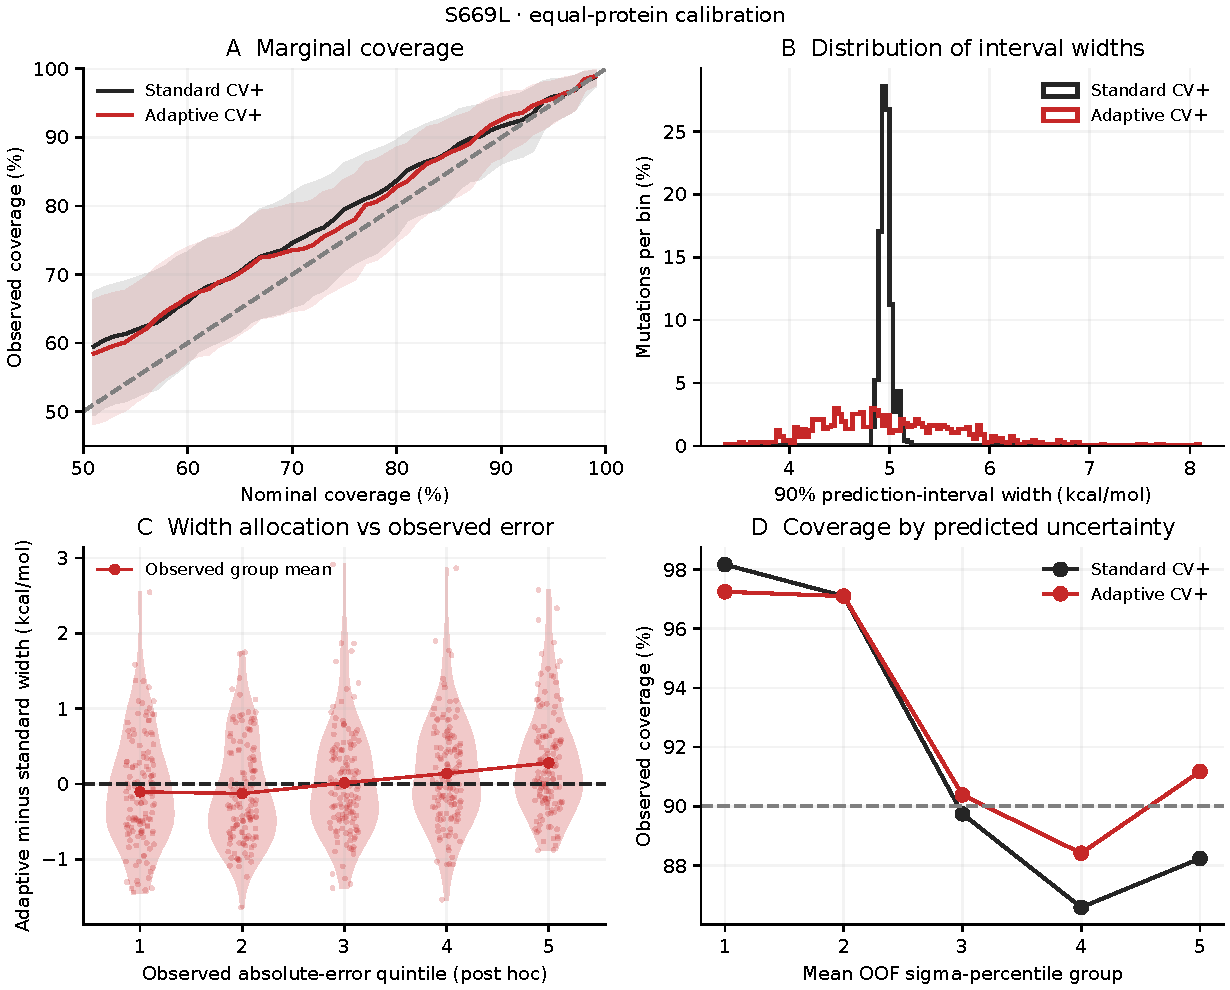
\includegraphics[width=0.96\textwidth]{s669l_uncertainty.pdf}
\caption{\textbf{What does predicted scale add to standard CV+ intervals?}
S669L results use the five nested-MSE refits, median point prediction and empirical
protein-weighted calibration from S2450. Black denotes standard and red adaptive CV+.
(A) Mutation-weighted observed versus nominal coverage at 49 levels (51--99\%), with
pointwise 95\% protein-cluster bootstrap bands (4,000 resamples).
(B) Distributions of both interval widths at nominal 90\%; standard CV+ is not exactly constant-width.
(C) Adaptive-minus-standard width in post-hoc quintiles of observed absolute median-prediction
error: violins and small points show mutations, connected large points show group means.
(D) Mutation-weighted coverage at 90\% within fixed uncertainty-percentile groups.
Groups in C are not used for calibration. The weighting of plotted external observations
is distinct from the equal-protein weighting used to construct intervals.}
\label{fig:uncertainty}
\end{figure*}

\begin{table*}[t]
\centering
\caption{Empirical performance of protein-weighted CV+ intervals at nominal 90\%.
Coverage is reported both per mutation and averaged equally over WT proteins.
Width and interval score (IS) are mutation-weighted and in $\kcal$; dispersion is the
population SD of mutation-weighted coverage across five predicted-uncertainty groups,
in percentage points.}
\label{tab:coverage}
\small
\begin{tabular}{llrrrrr}
\toprule
Dataset & Interval & Mutation coverage (\%) & Protein coverage (\%) & Mean width & IS & Dispersion\\
\midrule
S669L & Standard & 91.63 & 86.76 & 4.964 & 6.716 & 4.75\\
      & Adaptive & 92.53 & 86.87 & 5.004 & 6.551 & 3.63\\
S461L & Standard & 97.61 & 96.56 & 4.965 & 5.188 & 2.71\\
      & Adaptive & 98.05 & 93.85 & 4.967 & 5.109 & 1.47\\
\bottomrule
\end{tabular}
\end{table*}

\begin{figure*}[!tp]
\centering
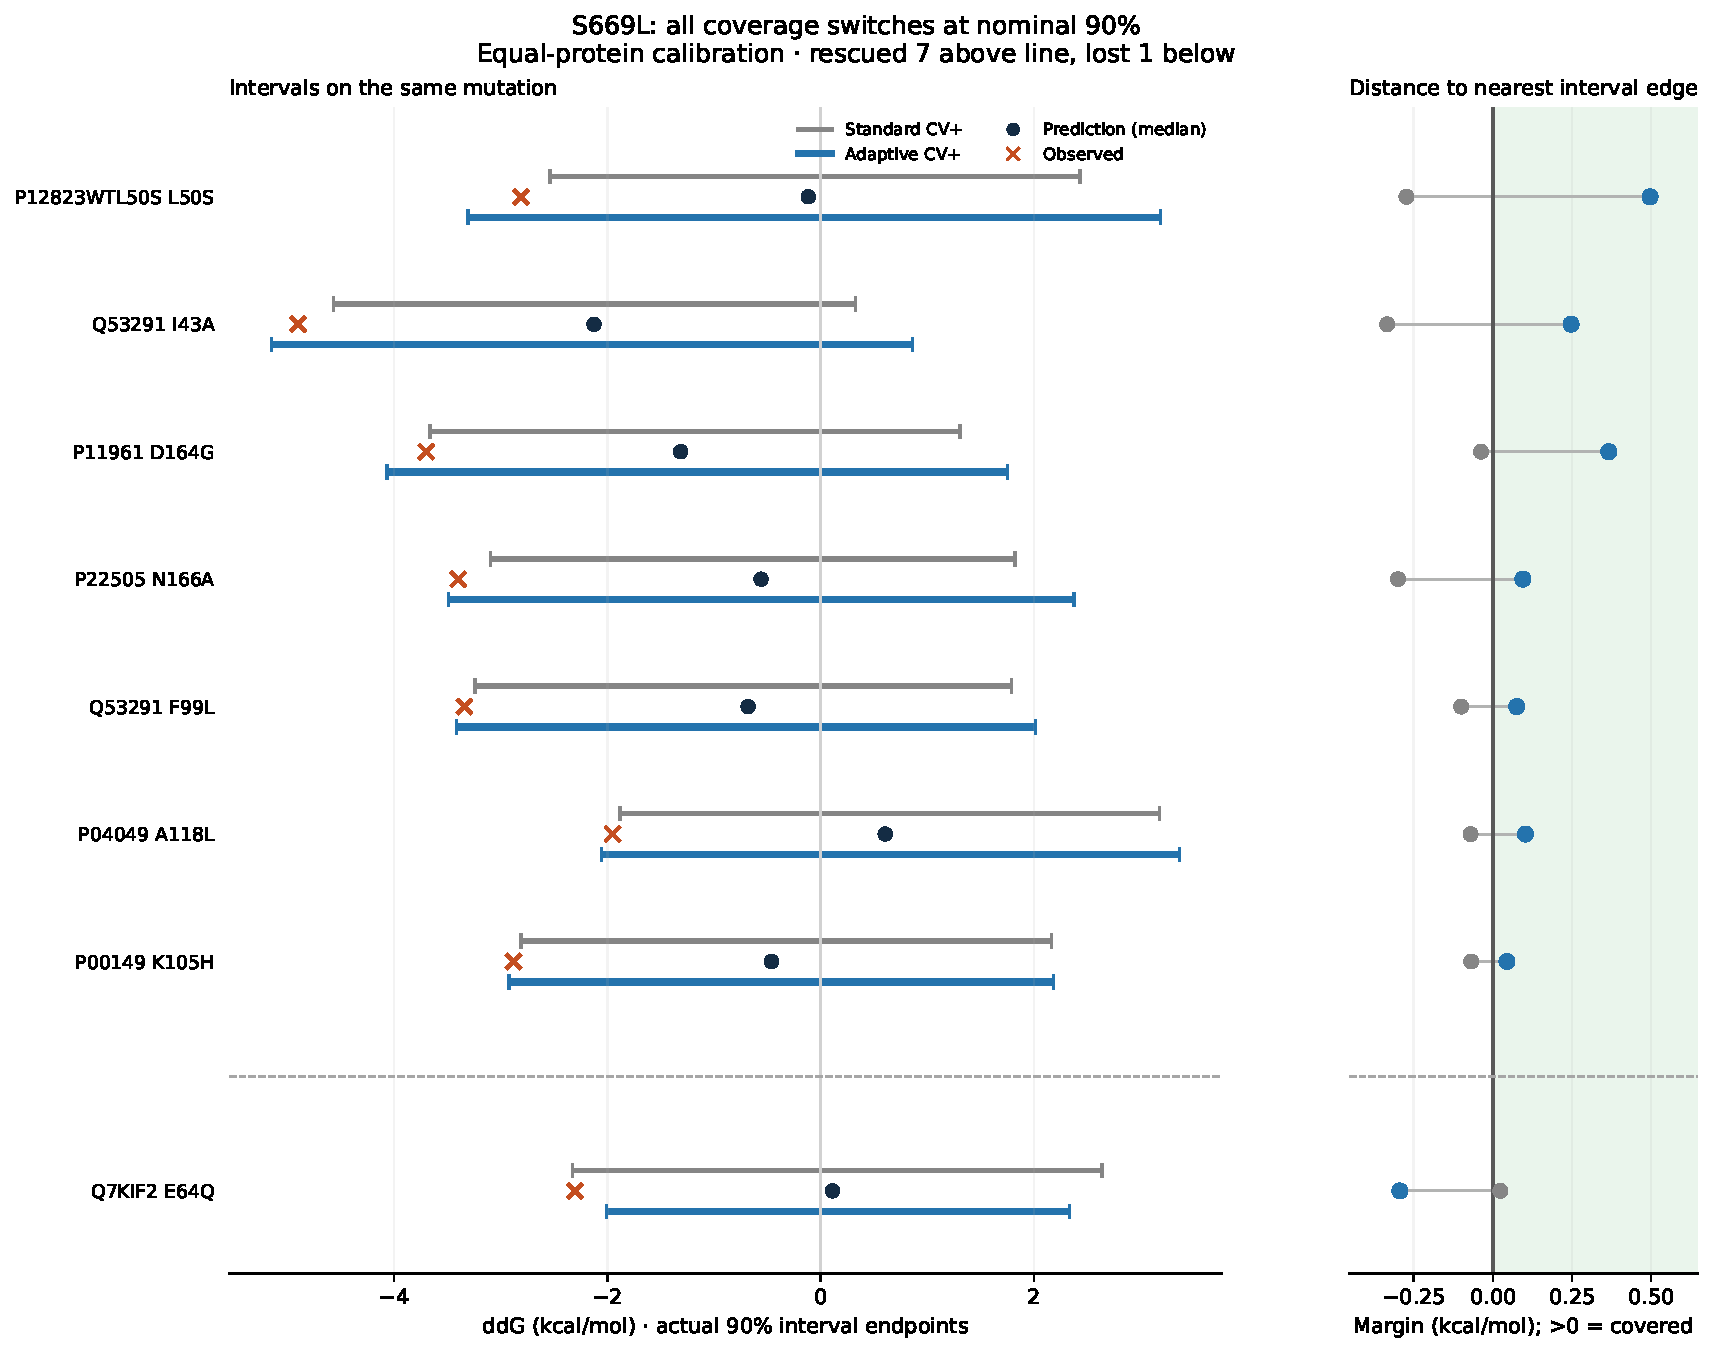
\includegraphics[width=0.94\textwidth]{s669l_coverage_switches.pdf}
\caption{All S669L coverage switches between the standard and adaptive protein-weighted
90\% intervals, using median point predictions. Seven rescued mutations are above the dashed
line and the single lost mutation is below. Left: true interval endpoints (gray standard,
blue adaptive), shared median prediction and measured target. Right: the signed margin
$\min(y-L,U-y)$, positive when covered and negative when missed. The cases are selected
post hoc by their coverage outcome and are illustrative rather than a performance estimate.}
\label{fig:switches}
\end{figure*}

% \subsubsection{Interval-based stabilizing and destabilizing calls}
% \label{sec:zero_exclusion}

% To quantify how often the predictive intervals identify the direction of a mutation stability change, we evaluated each integer nominal level $c$ from 50\% to 95\%, inclusive. For each level, we recomputed the adaptive empirical CV+ endpoints using the existing OOF residuals and equal-protein calibration weights, with $\alpha=1-c/100$.
% The model checkpoints and median point predictor were fixed.
% This analysis extends the coverage-curve grid to the 50\% nominal level under the same
% empirical weighted-quantile convention.

% Under our sign convention, a mutation is called stabilizing when the entire interval lies
% strictly above zero ($L_i(c)>0$), and destabilizing when it lies strictly below zero ($U_i(c)<0$). If the interval contains or touches zero, its direction is considered indeterminate at that nominal level. Thus the number of direction calls is
% \begin{equation}
% N_{\ne0}(c)=\sum_{i=1}^{N}\mathbf 1\{L_i(c)>0\ \text{or}\ U_i(c)<0\}.
% \end{equation}
% The mutation-level call rate is $100N_{\ne0}(c)/N$, using every mutation in the test set
% as the denominator, including indeterminate cases.

% Because several mutations belong to the same protein, we also count the distinct full-WT
% protein sequences with at least one direction call:
% \begin{equation}
% P_{\ge1}(c)=\sum_{p=1}^{P_{\rm test}}\mathbf 1\{\exists i\in p:
% L_i(c)>0\ \text{or}\ U_i(c)<0\}.
% \end{equation}
% Their percentage is $100P_{\ge1}(c)/P_{\rm test}$, with $P_{\rm test}=87$ for S669L and 46 for S461L. Each protein is counted once even if it contains multiple classified mutations or both stabilizing and destabilizing calls. This statistic does not assert that all mutations of that protein have a determined direction. Protein identifiers that map to the same full WT sequence are grouped together, consistently with calibration.

% Figure~\ref{fig:sign_exclusion} summarizes selected nominal levels; Appendix Table~\ref{tab:zero_exclusion} provides a more complete summary of the results across nominal coverage levels ranging from 50\% to 90\%.
% As representative low- and high-confidence settings, we focus here on the 50\% and 90\% nominal levels.
% At 50\%, 229 of 669 S669L mutations (34.23\%) and 190 of 461 S461L mutations (41.21\%)
% exclude zero, spanning 46 of 87 proteins (52.87\%) and 26 of 46 proteins (56.52\%),
% respectively. At 90\%, these counts fall to four mutations (0.60\%) from two proteins
% (2.30\%) on S669L, and five mutations (1.08\%) from two proteins (4.35\%) on S461L;
% all of these 90\% calls are destabilizing.  As the nominal level increases, the intervals expand and the set of direction calls can only shrink, a nesting property also checked numerically.

% For many practical applications, distinguishing whether a mutation is stabilizing or destabilizing can be more relevant than precisely estimating the magnitude of its \(\Delta\Delta G\). For this reason, we additionally report observed sign accuracy among the zero-excluding calls:
% \begin{equation}
% \begin{aligned}
% A_{\rm sign}(c)=\frac{100}{N_{\ne0}(c)}\sum_{i=1}^{N}\bigl[
% &\mathbf 1\{L_i(c)>0,\ y_i>0\}\\
% +{}&\mathbf 1\{U_i(c)<0,\ y_i<0\}\bigr].
% \end{aligned}
% \end{equation}
% Each called mutation contributes equally to this accuracy, independently of the
% protein weights used for calibration. An observed target equal to zero does not count
% as a correct directional call. Accuracy is undefined (shown as --) when no interval
% excludes zero. External targets are used only to evaluate sign accuracy, not to assign
% calls. Call rates and empirical sign accuracy are distinct from observed interval coverage
% and from probabilities that individual assigned signs are correct. In particular, a 90\% nominal interval does not establish 90\%
% accuracy among the selected mutations; such a selected-subset guarantee is not supplied
% by this empirical protein-weighted construction.

% \begin{figure*}[!t]
% \centering
% 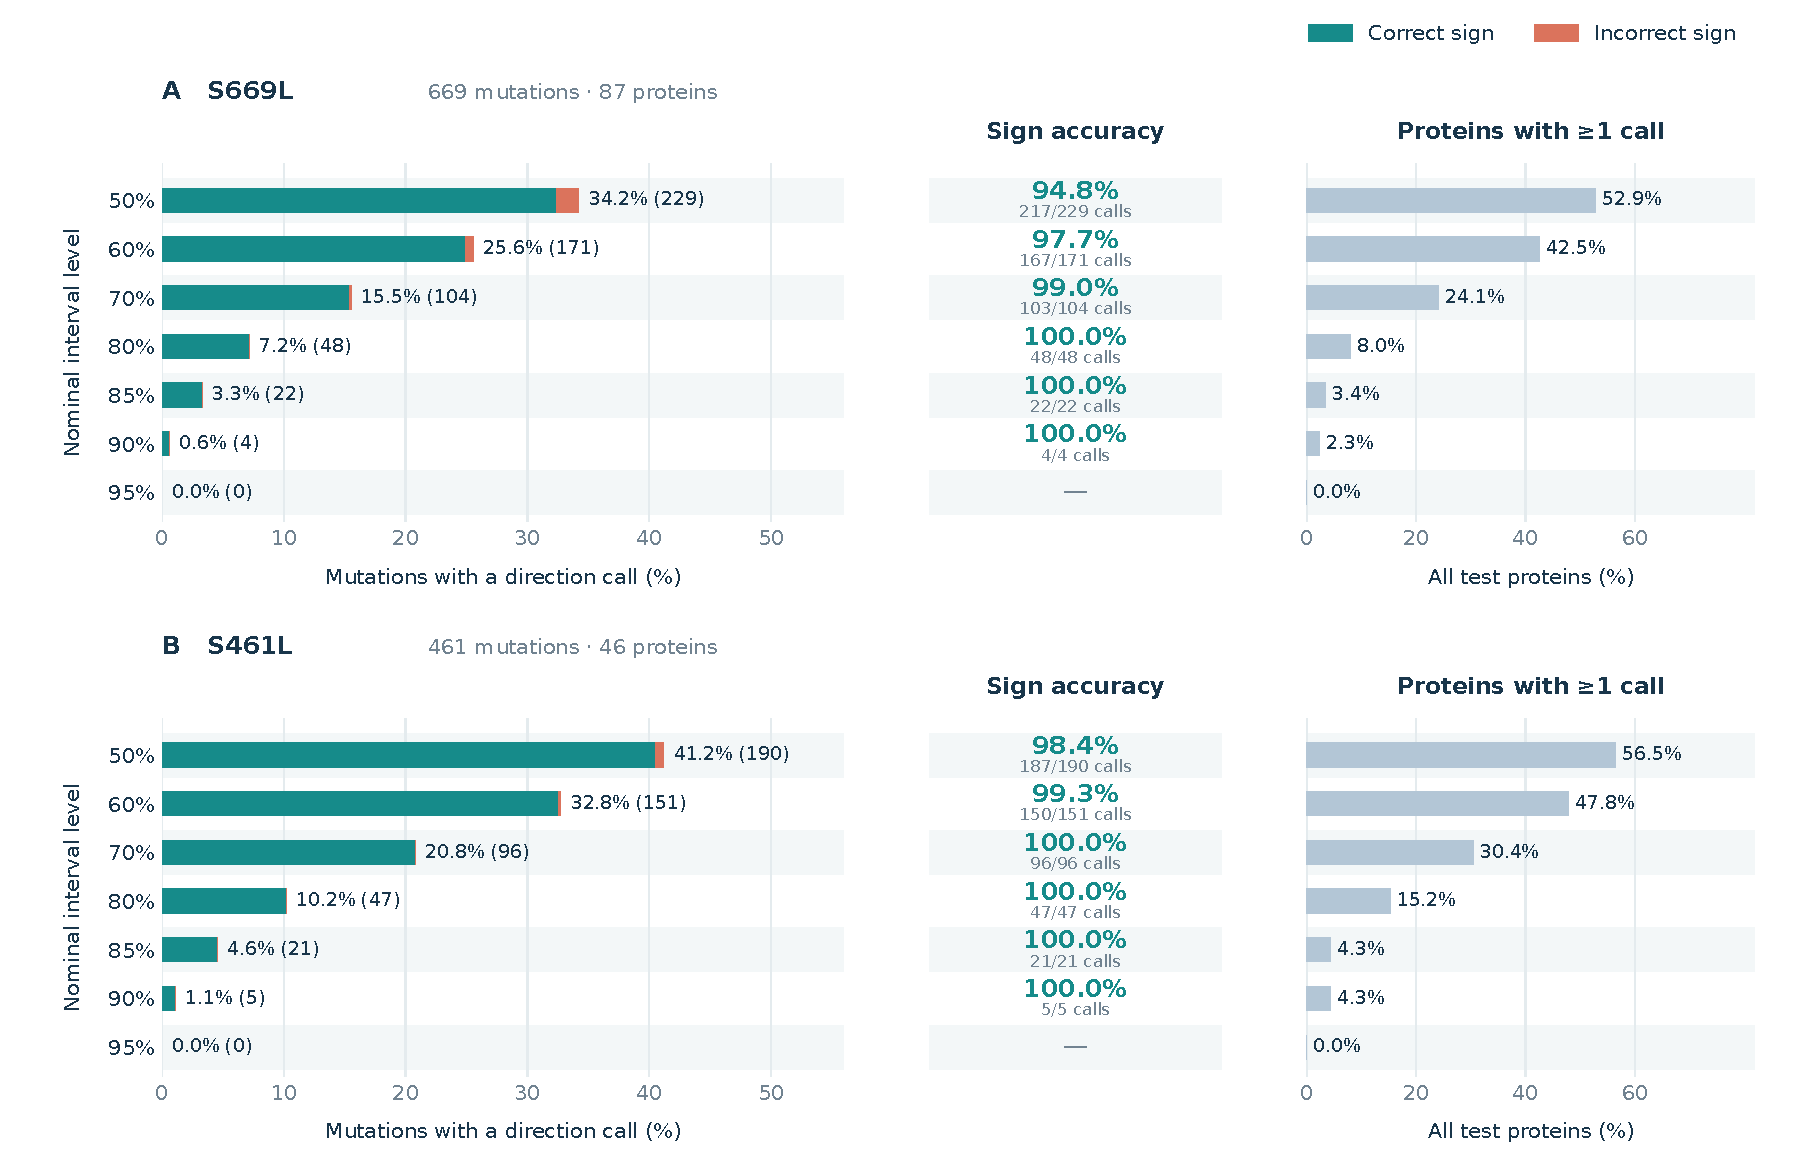
\includegraphics[width=\textwidth]{sign_exclusion_summary.pdf}
% \caption{Direction calls and observed sign accuracy for S669L (A) and S461L (B) at selected nominal interval levels. Calls are assigned when adaptive protein-weighted CV+ intervals lie strictly above or below zero. Left: percentage of all test mutations receiving a call, partitioned into correct and incorrect signs; labels give percentages and counts in parentheses. Center: observed sign accuracy among called mutations, with correct/total counts. Right: percentage of distinct full-WT proteins with at least one call. Calibration weights proteins equally, whereas sign accuracy weights called mutations equally. Observed zero targets count as incorrect; a dash indicates no calls. Empirical sign accuracy is not a nominal coverage guarantee. S461L overlaps S669L.}
% \label{fig:sign_exclusion}
% \end{figure*}


\subsubsection{Interval-based stabilizing and destabilizing calls}
\label{sec:zero_exclusion}

To quantify how often the predictive intervals identify the direction of  a mutation-induced stability change, we evaluated each integer nominal level $c$ from 50\% to 95\%, inclusive. For each level, we recomputed
the adaptive empirical CV+ endpoints using the existing OOF residuals and equal-protein calibration weights, with $\alpha=1-c/100$. The model checkpoints and median point predictor were fixed.
Evaluation used the original benchmark mutations without adding generated reverses, so each experimentally characterized mutation contributed once.

Under our sign convention, a mutation is called stabilizing when the entire interval lies strictly above zero ($L_i(c)>0$), and destabilizing when it lies strictly below zero ($U_i(c)<0$). If the interval contains or touches zero, its direction is considered indeterminate at that nominal level.
Thus the number of direction calls is
\begin{equation}
N_{\ne0}(c)=\sum_{i=1}^{N}\mathbf 1\{L_i(c)>0\ \text{or}\ U_i(c)<0\}.
\end{equation}
The mutation-level call rate is $100N_{\ne0}(c)/N$, using every mutation in the test set as the denominator, including indeterminate cases.

Because several mutations belong to the same protein, we also count the distinct full-WT protein sequences with at least one direction call:
\begin{equation}
P_{\ge1}(c)=\sum_{p=1}^{P_{\rm test}}\mathbf 1\{\exists i\in p:
L_i(c)>0\ \text{or}\ U_i(c)<0\}.
\end{equation}
Their percentage is $100P_{\ge1}(c)/P_{\rm test}$, with $P_{\rm test}=87$ for S669L and 46 for S461L. Each protein is counted once even if it contains multiple classified mutations or both stabilizing and destabilizing calls.
This statistic does not assert that all mutations of that protein have a determined direction. Protein identifiers that map to the same full WT sequence are grouped together, consistently with calibration.

Figure~\ref{fig:sign_exclusion} summarizes selected nominal levels and Supplementary Table~\ref{tab:zero_exclusion} provides a more complete summary of the results across nominal coverage levels ranging from 50\% to 90\%.
We highlight the 50\%, 70\%, and 90\% nominal levels to illustrate the relationship between call rate and observed sign accuracy.

At 50\%, 229 of 669 S669L mutations (34.23\%) and 190 of 461 S461L mutations (41.21\%) exclude zero, spanning 46 of 87 proteins (52.87\%) and 26 of 46 proteins (56.52\%), respectively.
Observed sign accuracy among these calls was 94.76\% (217/229) on S669L and 98.42\% (187/190) on S461L. At 70\%, the call rates decreased to 15.55\% (104/669) and 20.82\% (96/461), while sign accuracy increased to 99.04\% (103/104) and 100\% (96/96), respectively.
At 90\%, these counts fall to four mutations (0.60\%) from two proteins (2.30\%) on S669L, and five mutations (1.08\%) from two proteins (4.35\%) on S461L; all of these 90\% calls are destabilizing in the original benchmark orientation and have correct signs.
As the nominal level increases, the intervals expand and the set of direction calls can only shrink, a nesting property also checked numerically.

Most calls were destabilizing in the original benchmark orientation. Reversing a mutation changes the sign of the model's predicted $\Delta\Delta G$ while preserving its uncertainty scale. For a reflected interval $[-U_i(c),-L_i(c)]$, the directional call is likewise reversed, with unchanged correctness against the sign-inverted target. 

For many practical applications, distinguishing whether a mutation is stabilizing or destabilizing can be more relevant than precisely estimating the magnitude of its \(\Delta\Delta G\). For this reason, we additionally
report observed sign accuracy among the zero-excluding calls:
\begin{equation}
\begin{aligned}
A_{\rm sign}(c)=\frac{100}{N_{\ne0}(c)}\sum_{i=1}^{N}\bigl[
&\mathbf 1\{L_i(c)>0,\ y_i>0\}\\
+{}&\mathbf 1\{U_i(c)<0,\ y_i<0\}\bigr].
\end{aligned}
\end{equation}
Each called mutation contributes equally to this accuracy, independently of the protein weights used for calibration. An observed target equal to zero does not count as a correct directional call. Accuracy is undefined (shown as --) when no interval excludes zero. External targets are used only to evaluate sign accuracy, not to assign calls.
Call rates and empirical sign accuracy are distinct from observed interval coverage and from probabilities that individual assigned signs are correct.
In particular, a 90\% nominal interval does not establish 90\% accuracy among the selected mutations; such a selected-subset guarantee is not supplied by this empirical protein-weighted construction.

These results support zero-exclusion as a practical criterion for prioritizing mutations for experimental assessment: it identifies a subset with high observed directional accuracy while
abstaining on mutations whose intervals contain or touch zero.

\begin{figure*}[!t]
\centering
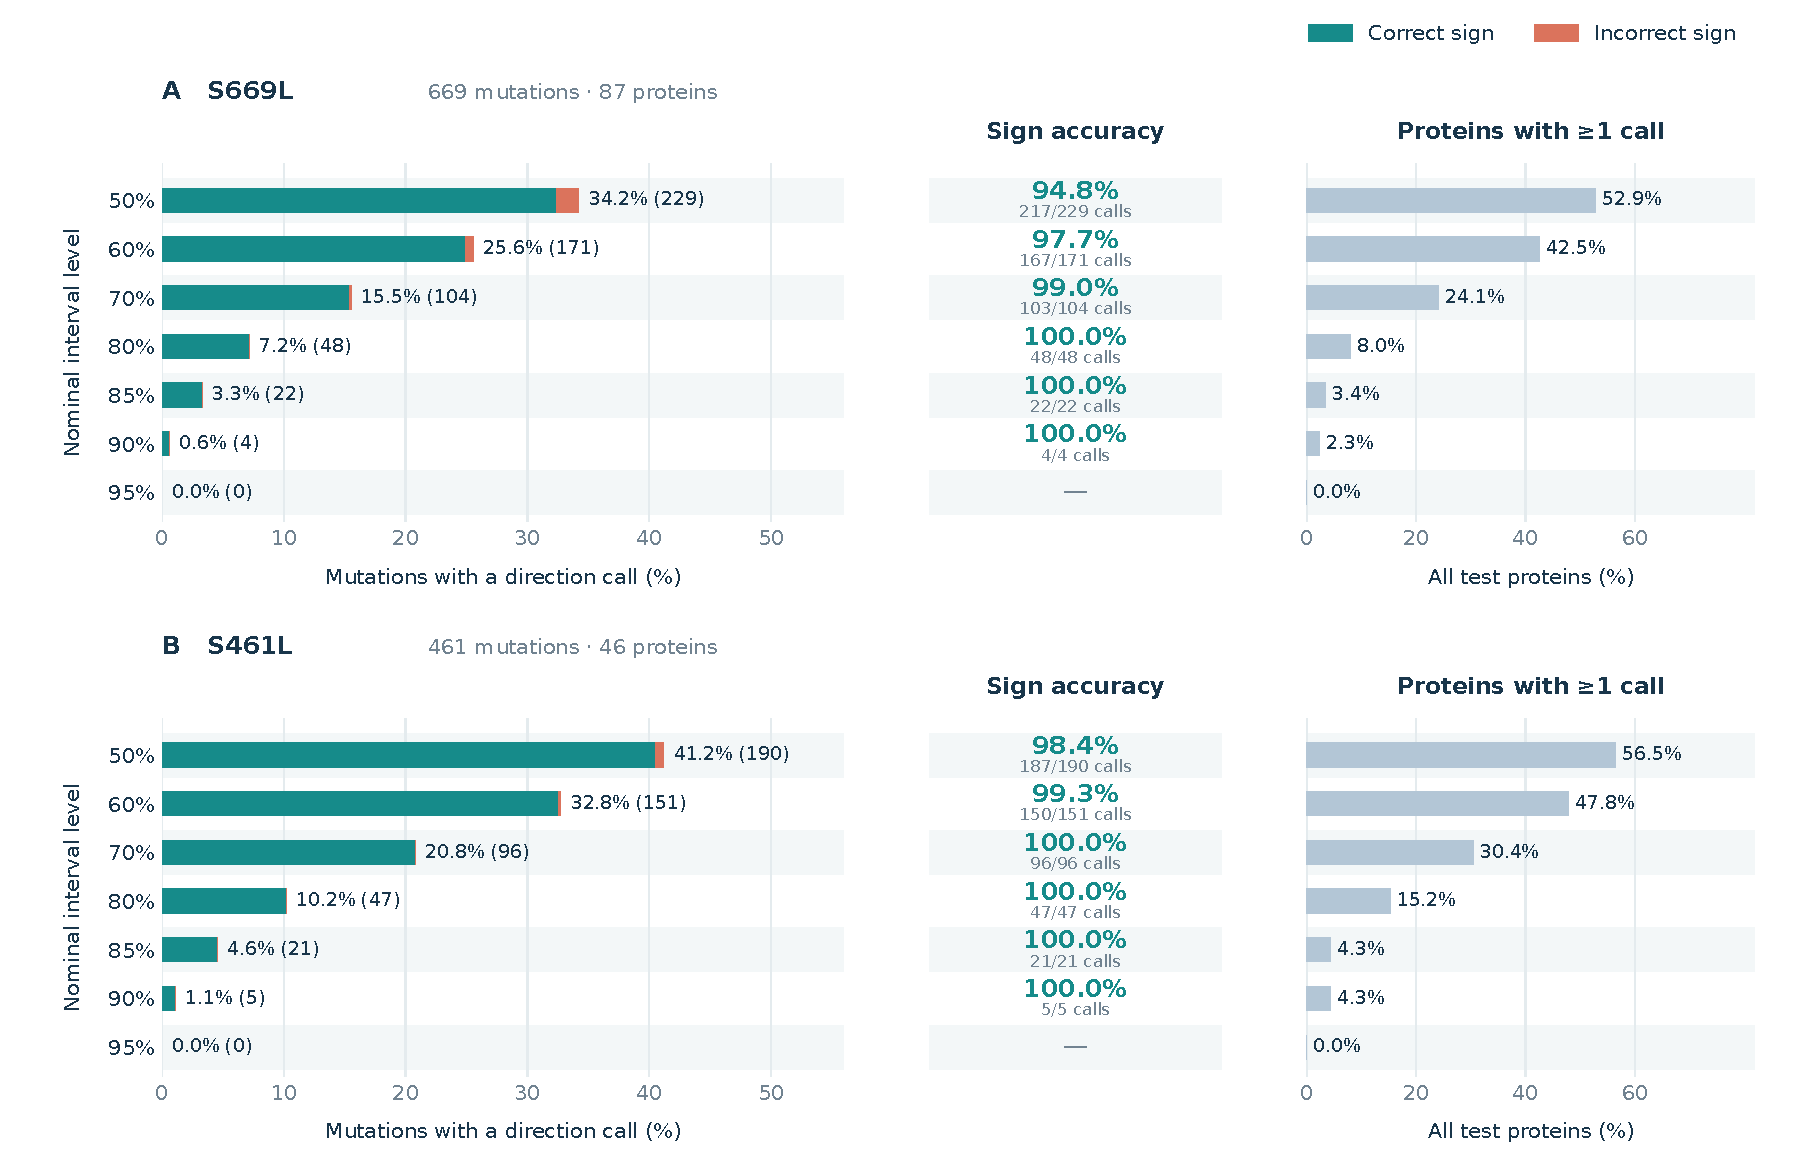
\includegraphics[width=\textwidth]{sign_exclusion_summary.pdf}
\caption{Direction calls and observed sign accuracy for S669L (A) and
S461L (B) at selected nominal interval levels.
Results use the original benchmark mutation directions,
without generated reverses.
Calls are assigned when adaptive protein-weighted CV+ intervals lie
strictly above or below zero.
Left: percentage of all test mutations receiving a call, partitioned
into correct and incorrect signs; labels give percentages and counts
in parentheses.
Center: observed sign accuracy among called mutations, with
correct/total counts.
Right: percentage of distinct full-WT proteins with at least one call.
Calibration weights proteins equally, whereas sign accuracy weights
called mutations equally. Observed zero targets count as incorrect;
a dash indicates no calls. Empirical sign accuracy is not a nominal
coverage guarantee. S461L overlaps S669L.}
\label{fig:sign_exclusion}
\end{figure*}

\subsubsection{Calibration with the baseline model}
\label{sec:naive_results}
To assess whether the calibration procedure transfers to a substantially different predictor, we evaluated the simple sequence-based baseline described above, which uses full-length one-hot encoded WT and mutant sequences without pretrained embeddings. In this comparison, both the input representation and model architecture are changed, while the training, validation, aggregation, and conformal calibration procedures are kept unchanged.

Point-prediction performance was lower than that of the main model. On S669L, the median
baseline prediction achieved Pearson $r=0.33$, Spearman $\rho=0.31$, MAE
$1.23\,\kcal$, and MSE $2.76\,(\mathrm{kcal\,mol^{-1}})^2$.
On S461L, the corresponding values were $r=0.43$, $\rho=0.40$, MAE
$1.00\,\kcal$, and MSE $1.74\,(\mathrm{kcal\,mol^{-1}})^2$.
Nevertheless, at the nominal 90\% level, standard and adaptive intervals covered
90.88\% and 90.28\% of S669L mutations, respectively
(Table~\ref{tab:naive_coverage}). Their mean widths were 5.64 and
$5.84\,\kcal$, compared with 4.96 and $5.00\,\kcal$ for ProbJanusDDG.
Coverage averaged equally across S669L proteins was lower, at 86.31\% and 86.41\%.
On S461L, mutation-level coverage was conservative for both interval rules, while
protein-averaged coverage was 91.59\% and 92.00\%.

\begin{table}[t]
\centering
\caption{One-hot baseline intervals at nominal 90\% coverage, using equal total
calibration weight per WT protein. Mutation coverage weights test mutations
equally; protein coverage averages within each WT protein and then equally across
proteins. Mean width weights test mutations equally and is expressed in
$\mathrm{kcal\,mol^{-1}}$. S461L overlaps S669L.}
\label{tab:naive_coverage}
\small
\begin{tabular}{llrrr}
\toprule
Dataset & Interval & Mutation  & Protein  & Width \\
\midrule
S669L & Standard & 90.88\% & 86.31\% & 5.64 \\
      & Adaptive & 90.28\% & 86.41\% & 5.84 \\
S461L & Standard & 95.88\% & 91.59\% & 5.64 \\
      & Adaptive & 96.31\% & 92.00\% & 5.93 \\
\bottomrule
\end{tabular}
\end{table}

These results support the practical applicability of the calibration procedure
across contrasting predictors: lower point accuracy can coexist with similar
mutation-level coverage, at the cost of wider intervals. The comparison therefore
separates the empirical calibration of intervals from the predictive information
that determines their usefulness and width.



\section{Discussion and Conclusions}

The results highlight several aspects of uncertainty modeling for mutation-induced
changes in protein stability. A first important point concerns thermodynamic reversal
symmetry. While the $\Delta\Delta G$ prediction is expected to change sign when the
mutation direction is reversed, the associated uncertainty should remain unchanged.
By enforcing these properties algebraically, the model guarantees consistency between
forward and reverse predictions and avoids contradictory uncertainty estimates for the
same mutation pair.

The learned scale also provides useful information about prediction reliability. Its
association with absolute prediction error is moderate, indicating that $\sigma$ should
not be interpreted as an accurate estimate of the error of an individual mutation.
Nevertheless, it captures some information about relative prediction difficulty.
This distinction is important in the conformal construction:
the predicted scale modulates the residual normalization and, consequently, the width
assigned to individual adaptive intervals, while empirical calibration 
sets the interval endpoints using held-out residuals.

More generally, our results show that marginal coverage alone does not fully describe
the behavior of mutation-specific prediction intervals. Standard and adaptive CV+
intervals can achieve similar overall coverage while distributing uncertainty
differently across mutations. In our experiments, adaptive intervals did not
systematically reduce mean width, nor did higher mutation-level coverage always
translate into improved protein-averaged coverage. Their main effect was instead to
redistribute interval width across predictions, with larger widening observed among
mutations with larger prediction errors, and to reduce coverage dispersion across
predicted-uncertainty groups. These findings support the joint evaluation of marginal
coverage, protein-level coverage, interval width, and coverage heterogeneity when
assessing uncertainty estimates for protein-stability predictors.

The directional-call analysis illustrates how these intervals can support decisions about which uncharacterized mutations to investigate experimentally.
When an interval lies entirely above or below zero, the method assigns a stabilizing
or destabilizing call; otherwise, it leaves the direction unresolved.
On S669L, this rule yielded 94.8\% observed sign accuracy for 34.2\% of mutations
at the 50\% nominal interval level, and 99.0\% accuracy for 15.5\% of mutations
at the 70\% level (Fig.~\ref{fig:sign_exclusion}).
Thus, highly accurate directional predictions were obtained for a substantial
subset, with higher nominal levels producing fewer calls.
These accuracies are empirical results among selected mutations, rather than
guarantees implied by the nominal interval levels.

For protein engineering, this criterion could help prioritize candidate stabilizing substitutions. For studies of protein function, it could identify candidate destabilizing variants for investigating effects mediated by changes in stability. In both settings, the intervals provide information beyond a point estimate by distinguishing mutations with a resolved predicted direction from those requiring further evidence. 
However, an interval containing zero does not establish that a mutation has a negligible effect, and excluding zero does not by itself establish a biologically important change or a functional consequence. 
Applications requiring a minimum stability change could instead compare the interval endpoints with a prespecified, biologically relevant effect-size threshold.

Application of the same calibration procedure to the one-hot sequence baseline illustrates its use across predictors with different representations and architectures. Together, these findings support conformal intervals as a complement to protein-stability point predictions and as a practical criterion for prioritizing uncharacterized mutations for experimental assessment.
Their usefulness should be assessed jointly through interval coverage, width, and the accuracy and frequency of directional calls.


% \section{Discussion}

% The results highlight several aspects of uncertainty modeling for mutation-induced
% changes in protein stability. A first important point concerns thermodynamic reversal
% symmetry. While the $\Delta\Delta G$ prediction is expected to change sign when the
% mutation direction is reversed, the associated uncertainty should remain unchanged.
% By enforcing these properties algebraically, the model guarantees consistency between
% forward and reverse predictions and avoids contradictory uncertainty estimates for the
% same mutation pair.

% The learned scale also provides useful information about prediction reliability. Its
% association with absolute prediction error is moderate, indicating that $\sigma$ should
% not be interpreted as an accurate estimate of the error of an individual mutation.
% Rather, it acts as a relative uncertainty signal that ranks predictions according to
% their expected reliability. This distinction is important in the conformal construction:
% the predicted scale modulates the residual normalization and, consequently, the width
% assigned to individual adaptive intervals, while empirical calibration determines the
% final coverage level.

% More generally, our results show that marginal coverage alone does not fully describe
% the behavior of mutation-specific prediction intervals. Standard and adaptive CV+
% intervals can achieve similar overall coverage while distributing uncertainty
% differently across mutations. In our experiments, adaptive intervals did not
% systematically reduce mean width, nor did higher mutation-level coverage always
% translate into improved protein-averaged coverage. Their main effect was instead to
% redistribute interval width across predictions, with larger widening observed among
% mutations with larger prediction errors, and to reduce coverage dispersion across
% predicted-uncertainty groups. These findings support the joint evaluation of marginal
% coverage, protein-level coverage, interval width, and coverage heterogeneity when
% assessing uncertainty estimates for protein-stability predictors.



% \section{Conclusion}

% In this work, we introduced a protein-stability predictor that combines $\Delta\Delta G$
% estimation with conformal prediction to provide calibrated, mutation-specific prediction
% intervals. The model produces an antisymmetric mean prediction together with a symmetric
% uncertainty estimate, while protein-weighted CV+ calibration limits the influence of
% proteins with many more observed mutations than others.

% Across external low-homology benchmarks, the proposed approach achieved point-prediction
% performance in line with the current state of the art and produced empirical interval
% coverage close to the nominal levels. The adaptive formulation redistributed interval
% width across mutations while maintaining a similar average width to standard CV+, and
% the learned scale showed a positive association with observed prediction error. In
% addition, the resulting intervals provide a direct practical criterion for assessing
% whether the predicted effect of an individual mutation remains unambiguously stabilizing
% or destabilizing at a given confidence level.

% The same calibration procedure was also successfully applied to a deliberately simple one-hot sequence model, illustrating that the conformal component is not tied to a specific predictive architecture or representation and could therefore be incorporated into future protein-stability predictors to provide calibrated uncertainty estimates. Overall, these results show that
% conformal prediction provides a practical route to complement protein-stability point
% predictions with interpretable uncertainty estimates, while also emphasizing the
% importance of evaluating coverage at both the mutation and protein levels.

\section*{Acknowledgements}
To be completed.


\section*{Funding}
To be completed.

\section*{Competing interests}
The authors declare no competing interests.



\clearpage
\appendix
\onecolumn

\section{Supplementary}

\subsection{Method performance on external datasets}
\label{app:performance}


To place the predictive performance of ProbJanusDDG in the context of existing
$\Delta\Delta G$ predictors, we compared its point-prediction accuracy with that of
recent state-of-the-art methods on the external S669L and S461L benchmarks. The
comparison includes both sequence-based and structure-based approaches, allowing
ProbJanusDDG to be evaluated against methods that differ substantially in input
representation, architecture, and use of structural information.

Performance was assessed using the same external test sets adopted in the main
analysis. For ProbJanusDDG, predictions correspond to the median ensemble output
across the five refitted models. The benchmark metrics considered were Pearson
correlation and mean absolute error (MAE), whenever the corresponding values were available for the reference
methods. The complete comparison is reported in Supplementary
Table~\ref{tab:point}.

On S669L, ProbJanusDDG achieved predictive performance comparable to the strongest
methods reported for this low-homology benchmark, indicating that the introduction
of uncertainty estimation and conformal calibration does not come at the expense of
competitive point-prediction accuracy. On S461L, performance was higher across the
main regression metrics, further supporting the ability of the model to generalize
to an independently curated external set.

Overall, these results show that ProbJanusDDG remains competitive with current
state-of-the-art protein-stability predictors while additionally providing
mutation-specific uncertainty estimates and calibrated prediction intervals, which
are not available from most conventional $\Delta\Delta G$ prediction methods.




\begin{table}[h]
\centering
\caption{Point-prediction performance of the median ensemble on the external test sets.}
\label{tab:point_prediction_performance}
\small
\begin{tabular}{lcccc}
\toprule
Dataset & Pearson $r$ & Spearman $\rho$ & MAE & MSE \\
\midrule
S669L & $0.53$ & $0.55$ & $0.99$ & $2.03$ \\
S461L & $0.70$ & $0.68$ & $0.74$ & $0.97$ \\
\bottomrule
\end{tabular}
\vspace{2pt}

\end{table}



\begin{table*}[h]
\centering
\caption{Point-prediction performance on the external S669 and S461
benchmarks. Comparative values and the original JanusDDG results are taken
from the source data of Fig.~3 of the JanusDDG paper. ProbJanusDDG denotes
the median of the five models selected by protein-weighted MSE and refitted on four folds. Its rows use the local S669L and S461L datasets. MAE is reported in \(\mathrm{kcal\,mol^{-1}}\). The S461 values refer to the
direct-mutation evaluation.}
\label{tab:point}
\scriptsize
\setlength{\tabcolsep}{3.5pt}
\begin{minipage}[t]{0.485\textwidth}
\centering
\textbf{S669}\\[2pt]
\begin{tabular}{lcc}
\toprule
Model & Pearson \(r\) & MAE \\
\midrule
JanusDDG          & 0.55 & 0.97 \\
DDGemb            & 0.53 & 0.99 \\
MAESTRO           & 0.50 & 1.06 \\
PROSTATA          & 0.49 & 1.00 \\
ACDC-NN           & 0.46 & 1.05 \\
DDGun3D           & 0.43 & 1.11 \\
INPS3D            & 0.43 & 1.07 \\
INPS-Seq          & 0.43 & 1.09 \\
ACDC-NN-Seq       & 0.42 & 1.08 \\
SDM               & 0.41 & 1.26 \\
DUET              & 0.41 & 1.10 \\
DynaMut           & 0.41 & 1.19 \\
PoPMuSiC          & 0.41 & 1.09 \\
DDGun             & 0.41 & 1.25 \\
PremPS            & 0.41 & 1.08 \\
ThermoNet         & 0.39 & 1.17 \\
THPLM             & 0.39 & --   \\
Rosetta           & 0.39 & 2.08 \\
mCSM              & 0.36 & 1.13 \\
I-Mutant3.0       & 0.36 & 1.12 \\
SAAFEC-SEQ        & 0.36 & 1.13 \\
I-Mutant3.0-Seq   & 0.34 & 1.15 \\
DynaMut2          & 0.34 & 1.15 \\
MUpro             & 0.25 & 1.21 \\
FoldX             & 0.22 & 1.56 \\
\midrule
\textbf{ProbJanusDDG (CV+ median)} & \textbf{0.530} & \textbf{0.993} \\
\bottomrule
\end{tabular}
\end{minipage}\hfill
\begin{minipage}[t]{0.485\textwidth}
\centering
\textbf{S461}\\[2pt]
\begin{tabular}{lcc}
\toprule
Model & Pearson \(r\) & MAE \\
\midrule
JanusDDG           & 0.69 & 0.71 \\
PremPS             & 0.63 & 0.80 \\
MAESTRO            & 0.63 & 0.79 \\
DDGun3D            & 0.63 & 0.81 \\
stability-oracle   & 0.62 & 0.89 \\
PoPMuSiC           & 0.61 & 0.76 \\
INPS3D             & 0.61 & 0.76 \\
CartddgD           & 0.60 & 2.93 \\
ACDC-NN            & 0.60 & 0.78 \\
DUET               & 0.59 & 0.78 \\
KORPMD             & 0.57 & 0.91 \\
SDM                & 0.56 & 1.02 \\
ThermoNet          & 0.55 & 0.93 \\
mCSM               & 0.53 & 0.81 \\
DynaMut            & 0.50 & 0.96 \\
I-Mutant3.0        & 0.49 & 0.84 \\
SAAFEC-Seq         & 0.49 & 0.84 \\
mif                & 0.45 & 3.14 \\
ankh               & 0.44 & 4.69 \\
esm2-650M          & 0.43 & 3.55 \\
mpnn-20-00         & 0.40 & 1.88 \\
esm1v-mean         & 0.39 & 3.33 \\
esmif-multimer     & 0.37 & 1.26 \\
mifst              & 0.37 & 3.95 \\
mutcomputex        & 0.33 & 1.03 \\
FoldXD             & 0.30 & 1.26 \\
MSA-Transformer   & 0.30 & 5.05 \\
Tranception        & 0.24 & 1.29 \\
\midrule
\textbf{ProbJanusDDG (CV+ median)} & \textbf{0.704} & \textbf{0.736} \\
\bottomrule
\end{tabular}
\end{minipage}
\end{table*}


% \subsection{Conformal prediction}

% Conformal prediction provides a distribution-free framework for constructing prediction sets with finite-sample marginal coverage under exchangeability, i.e.,

% $$
% (Z_1,\ldots,Z_n)
% \overset{d}{=}
% (Z_{\pi(1)},\ldots,Z_{\pi(n)})
% $$

% for every permutation \(\pi\) of \(\{1,\ldots,n\}\), meaning that the joint distribution of the observations is invariant to their ordering.


% In regression, the general idea is to quantify the discrepancy between the observed target and the model prediction through a nonconformity score, i.e., a measure of how atypical an observation is relative to the model prediction, and then use the empirical distribution of these scores to determine the width of a prediction interval.

% We first describe split conformal prediction as background, then distinguish the CV+ construction used here and its empirical protein-weighted extension.


% \paragraph{Split conformal prediction.}
% Consider a regression model trained on a proper training set and a disjoint calibration set
% \begin{equation}
% \mathcal{C}=\{(x_i,y_i)\}_{i=1}^{n}.
% \end{equation}
% Let \(\mu(x)\) denote the point prediction produced by the fitted model. A standard nonconformity score is the absolute residual
% \begin{equation}
% r_i = |y_i-\mu(x_i)|.
% \end{equation}
% Let
% \begin{equation}
% r_{(1)} \leq r_{(2)} \leq \cdots \leq r_{(n)}.
% \end{equation}
% denote the ordered calibration scores. For a desired marginal coverage level \(1-\alpha\), the conformal threshold is given by
% \begin{equation}
% q_{1-\alpha}
% =
% r_{(k)},
% \qquad
% k=
% \left\lceil (n+1)(1-\alpha)\right\rceil,
% \end{equation}
% with an additional score $r_{(n+1)}=+\infty$ if $k=n+1$; truncating the index at $n$ would not in general preserve the stated guarantee.

% The resulting prediction interval for a new input \(x\) is
% \begin{equation}
% C_{1-\alpha}(x)
% =
% \left[
% \mu(x)-q_{1-\alpha},
% \mu(x)+q_{1-\alpha}
% \right].
% \end{equation}

% Under exchangeability of the calibration observations and the future test observation, and provided that the fitted predictor is independent of the calibration targets, split conformal prediction satisfies the finite-sample marginal coverage guarantee
% \begin{equation}
% \mathbb{P}
% \left[
% Y_{n+1}
% \in
% C_{1-\alpha}(X_{n+1})
% \right]
% \geq
% 1-\alpha.
% \end{equation}
% This guarantee is distribution-free and does not require the predictive model or the residuals to follow a specific parametric distribution. It is, however, a marginal rather than conditional guarantee: coverage is ensured on average over future observations, rather than separately for every possible input \(x\).

% Intervals based on absolute residuals have a common half-width \(q_{1-\alpha}\) for all test samples. This can be inefficient in heteroscedastic settings, where prediction errors vary systematically across inputs. Adaptive conformal intervals can instead be obtained by normalizing the residuals by a positive, input-dependent scale \(\sigma(x)\), which may be predicted directly as an additional output of the model.

% The calibration scores are then defined as
% \begin{equation}
% r_i
% =
% \frac{|y_i-\mu(x_i)|}
% {\sigma(x_i)}.
% \end{equation}

% This normalization can be interpreted as expressing the prediction error relative to the model-estimated uncertainty for each sample. In the idealized case where the residuals can be written as \(Y-\mu(X)=\sigma(X)\varepsilon\), with \(\varepsilon\) following a common distribution across inputs, dividing by \(\sigma(X)\) removes the input-dependent scale of the errors, yielding normalized scores with a more homogeneous distribution across samples. Importantly, conformal validity does not require this factorization to hold exactly, nor does \(\sigma(x)\) need to be a perfectly calibrated conditional standard deviation; validity requires a positive scale fixed independently of calibration targets. A useful ranking of prediction difficulty concerns interval efficiency, not the existence of the split-conformal guarantee.



% After computing the conformal quantile \(q_{1-\alpha}\) from the normalized calibration scores, the prediction interval becomes
% \begin{equation}
% C_{1-\alpha}(x)
% =
% \left[
% \mu(x)-q_{1-\alpha}\sigma(x),
% \mu(x)+q_{1-\alpha}\sigma(x)
% \right].
% \end{equation}

% Equivalently, a future observation is contained in the interval whenever
% \begin{equation}
% \frac{|Y-\mu(X)|}
% {\sigma(X)}
% \leq
% q_{1-\alpha}.
% \end{equation}

% In this formulation, \(\sigma(x)\) determines how interval width varies across samples, whereas \(q_{1-\alpha}\) provides a global calibration factor estimated from held-out data. If larger values of \(\sigma(x)\) reliably correspond to samples with larger expected prediction errors, normalized conformal prediction can produce substantially more adaptive intervals than those based on unscaled residuals.

% \paragraph{CV+ and model-specific prediction candidates.}
% In data-limited settings, CV+ avoids reserving a separate calibration set by reusing the available observations through \(K\)-fold cross-validation \citep{barber2021jackknife}. Let

% $$
% \mathcal I_1,\ldots,\mathcal I_K
% $$

% denote a partition of the \(n\) observations into \(K\) folds. For each fold \(k\), let

% $$
% \widehat f^{-k}
% \qquad\text{and}\qquad
% \widehat\sigma^{-k}
% $$

% denote the prediction and scale models fitted using all observations except those belonging to \(\mathcal I_k\).

% For an observation \(i\in\mathcal I_k\), we compute the normalized out-of-fold nonconformity score

% $$
% S_i
% =
% \frac{
% \left|Y_i-\widehat f^{-k}(X_i)\right|
% }{
% \widehat\sigma^{-k}(X_i)
% }.
% $$

% Because observation \(i\) is not used to fit either \(\widehat f^{-k}\) or \(\widehat\sigma^{-k}\), \(S_i\) is an out-of-fold measure of prediction error relative to the local error scale estimated by the same fitted model.

% The defining feature of CV+ is that the score \(S_i\) remains paired with the fold-specific model that generated it when constructing a prediction interval for a new input \(x\). For \(i\in\mathcal I_k\), consider the candidate conformity condition

% $$
% \frac{
% \left|y-\widehat f^{-k}(x)\right|
% }{
% \widehat\sigma^{-k}(x)
% }
% \le S_i.
% $$

% Assuming

% $$
% \widehat\sigma^{-k}(x)>0,
% $$

% this condition is equivalent to

% $$
% \left|y-\widehat f^{-k}(x)\right|
% \le
% S_i\,\widehat\sigma^{-k}(x),
% $$

% and hence to

% $$
% \widehat f^{-k}(x)
% -
% S_i\,\widehat\sigma^{-k}(x)
% \le y\le
% \widehat f^{-k}(x)
% +
% S_i\,\widehat\sigma^{-k}(x).
% $$

% Each observation therefore contributes a pair of model-specific candidate endpoints,

% $$
% L_i(x)
% =
% \widehat f^{-k(i)}(x)
% -
% S_i\,\widehat\sigma^{-k(i)}(x),
% $$

% $$
% U_i(x)
% =
% \widehat f^{-k(i)}(x)
% +
% S_i\,\widehat\sigma^{-k(i)}(x),
% $$

% where \(k(i)\) denotes the fold containing observation \(i\).

% This pairing is the key distinction between CV+ and a procedure that first estimates a distribution of cross-validation residuals and then applies a single residual quantile to a separate model fitted on all observations. CV+ instead preserves the association

% $$
% \left(
% S_i,\,
% \widehat f^{-k(i)}(x),\,
% \widehat\sigma^{-k(i)}(x)
% \right),
% $$

% so that the uncertainty contribution associated with observation \(i\) is evaluated relative to the same fitted model that produced its out-of-fold score.

% In the standard unweighted construction, the lower and upper prediction limits are obtained by aggregating the candidate endpoints through empirical quantiles. Writing

% $$
% \tau_n
% =
% (1-\alpha)\left(1+\frac{1}{n}\right),
% $$

% the interval can be expressed as

% \[
% \begin{aligned}
% C_\alpha^{\mathrm{CV+}}(x)
% =\Big[&-Q_{\tau_n}\big(-L_1(x),\ldots,-L_n(x)\big),\\
%       &Q_{\tau_n}\big(U_1(x),\ldots,U_n(x)\big)\Big].
% \end{aligned}
% \]

% where \(Q_{\tau_n}\) denotes the finite-sample empirical quantile used in CV+.

% Thus CV+ does not aggregate the scores \(S_i\) first and then center a single interval around a refitted predictor. Instead, it first constructs the observation-specific quantities

% $$
% \widehat f^{-k(i)}(x)
% \pm
% S_i\,\widehat\sigma^{-k(i)}(x)
% $$

% and only afterwards aggregates these candidate endpoints. Consequently, both the variability of the out-of-fold scores and the variability among the fold-specific fitted models contribute to the final prediction interval.

% In our application, mutations are nested within proteins, and proteins contribute different numbers of mutations. Using ordinary empirical quantiles would therefore give greater total influence to proteins with more measured mutations. We retain the CV+ pairing between each out-of-fold score and its corresponding fold-specific prediction candidate, but replace the standard equal-mutation empirical quantiles by weighted empirical quantiles that assign the same total mass to each protein.

% Let \(G\) denote the total number of proteins represented in the calibration data. For each observation \(i\), let \(g(i)\in\{1,\ldots,G\}\) denote the protein to which observation \(i\) belongs, and let \(n_g\) denote the number of observed mutations associated with protein \(g\).

% To assign the same total weight to each protein, observation \(i\) is given weight

% $$
% w_i
% =
% \frac{1}{G\,n_{g(i)}}.
% $$

% Indeed, the total weight assigned to protein \(g\) is

% $$
% \sum_{i:\,g(i)=g} w_i
% =
% n_g\frac{1}{G n_g}
% =
% \frac{1}{G}.
% $$

% Thus, each protein contributes equally to the weighted empirical distribution, regardless of how many mutations are observed for that protein.


% so that each protein has total weight

% $$
% \sum_{i:g(i)=g}w_i
% =
% \frac{1}{G}.
% $$

% If \(Q_\tau^{(w)}\) denotes the weighted empirical quantile,

% $$
% Q_\tau^{(w)}(z_1,\ldots,z_n)
% =
% \inf
% \left\{
% z:
% \sum_{i=1}^n
% w_i\mathbf 1\{z_i\le z\}
% \ge \tau
% \right\},
% $$

% the resulting protein-balanced interval is

% $$
% \begin{aligned}
% C_\alpha^{\mathrm{wCV+}}(x)
% =
% \Bigg[
% &-
% Q_{\tau}^{(w)}
% \left(
% -L_1(x),\ldots,-L_n(x)
% \right),\\
% &
% Q_{\tau}^{(w)}
% \left(
% U_1(x),\ldots,U_n(x)
% \right)
% \Bigg].
% \end{aligned}
% $$


% This modification preserves the model-specific score--prediction pairing of CV+ while changing the empirical measure used to aggregate candidate endpoints. Unequal weighting is compatible with finite-sample conformal guarantees under appropriate conditions; weighted conformal and weighted CV+ constructions have been developed for settings in which the weights are linked to the sampling or train--test distributional structure. Our equal-protein weights assign each protein the same total calibration mass, thereby targeting a protein-balanced rather than mutation-balanced empirical distribution. The validity guarantee therefore depends on whether this weighting scheme can be identified with the appropriate weighting induced by the target sampling distribution. We state the corresponding sampling assumptions below.



\subsection{Direction calls at all nominal levels}
\label{app:direction_calls}

Table~\ref{tab:zero_exclusion}
summarizes the results at selected nominal coverage levels between 50\% and 90\%, providing the numerical values corresponding to Fig.~\ref{fig:sign_exclusion}.




\begin{table*}
\centering
\caption{Direction calls from adaptive protein-weighted CV+ intervals at each nominal level. $N_+$ and $N_-$ count intervals strictly above and strictly below zero. $N_{\ne0}$ is their sum; its percentage uses all test mutations (669 or 461). $P_{\ge1}$ counts distinct WT proteins with at least one such mutation; its percentage uses all test proteins (87 or 46). Proteins can have both types of mutation and are counted once in $P_{\ge1}$. Sign acc. is the percentage of zero-excluding calls whose assigned sign matches the observed target, with equal weight per called mutation. Zero targets count as incorrect; -- denotes no calls. This empirical accuracy is distinct from nominal coverage.}
\label{tab:zero_exclusion}
\small
\setlength{\tabcolsep}{3pt}
\renewcommand{\arraystretch}{1.04}
\begin{tabular}{r rrrrr rrrrr}
\toprule
& \multicolumn{5}{c}{S669L: 669 mutations, 87 proteins} & \multicolumn{5}{c}{S461L: 461 mutations, 46 proteins}\\
\cmidrule(lr){2-6}\cmidrule(lr){7-11}
Nominal (\%) & $N_+$ & $N_-$ & $N_{\ne0}$ (\%) & $P_{\ge1}$ (\%) & Sign acc. (\%) & $N_+$ & $N_-$ & $N_{\ne0}$ (\%) & $P_{\ge1}$ (\%) & Sign acc. (\%)\\
\midrule
50 & 10 & 219 & 229 (34.23) & 46 (52.87) & 94.76 & 7 & 183 & 190 (41.21) & 26 (56.52) & 98.42\\
% 51 & 9 & 213 & 222 (33.18) & 44 (50.57) & 96.40 & 7 & 181 & 188 (40.78) & 26 (56.52) & 98.94\\
% 52 & 7 & 208 & 215 (32.14) & 44 (50.57) & 96.28 & 5 & 176 & 181 (39.26) & 25 (54.35) & 98.90\\
% 53 & 7 & 201 & 208 (31.09) & 43 (49.43) & 96.63 & 5 & 172 & 177 (38.39) & 25 (54.35) & 98.87\\
% 54 & 6 & 197 & 203 (30.34) & 41 (47.13) & 96.55 & 4 & 169 & 173 (37.53) & 23 (50.00) & 98.84\\
55 & 6 & 195 & 201 (30.04) & 41 (47.13) & 96.52 & 4 & 167 & 171 (37.09) & 23 (50.00) & 98.83\\
% 56 & 6 & 186 & 192 (28.70) & 39 (44.83) & 96.35 & 4 & 163 & 167 (36.23) & 23 (50.00) & 98.80\\
% 57 & 5 & 183 & 188 (28.10) & 39 (44.83) & 96.28 & 3 & 159 & 162 (35.14) & 23 (50.00) & 98.77\\
% 58 & 5 & 175 & 180 (26.91) & 39 (44.83) & 96.67 & 3 & 154 & 157 (34.06) & 23 (50.00) & 98.73\\
% 59 & 5 & 171 & 176 (26.31) & 38 (43.68) & 97.16 & 3 & 150 & 153 (33.19) & 22 (47.83) & 99.35\\
60 & 3 & 168 & 171 (25.56) & 37 (42.53) & 97.66 & 3 & 148 & 151 (32.75) & 22 (47.83) & 99.34\\
% 61 & 3 & 160 & 163 (24.36) & 34 (39.08) & 97.55 & 2 & 141 & 143 (31.02) & 20 (43.48) & 100.00\\
% 62 & 2 & 156 & 158 (23.62) & 33 (37.93) & 97.47 & 2 & 136 & 138 (29.93) & 20 (43.48) & 100.00\\
% 63 & 2 & 153 & 155 (23.17) & 33 (37.93) & 97.42 & 2 & 133 & 135 (29.28) & 20 (43.48) & 100.00\\
% 64 & 2 & 148 & 150 (22.42) & 33 (37.93) & 97.33 & 2 & 130 & 132 (28.63) & 20 (43.48) & 100.00\\
65 & 2 & 135 & 137 (20.48) & 29 (33.33) & 98.54 & 2 & 120 & 122 (26.46) & 18 (39.13) & 100.00\\
% 66 & 2 & 131 & 133 (19.88) & 29 (33.33) & 99.25 & 2 & 119 & 121 (26.25) & 18 (39.13) & 100.00\\
% 67 & 2 & 124 & 126 (18.83) & 26 (29.89) & 99.21 & 2 & 115 & 117 (25.38) & 17 (36.96) & 100.00\\
% 68 & 2 & 117 & 119 (17.79) & 24 (27.59) & 99.16 & 2 & 109 & 111 (24.08) & 17 (36.96) & 100.00\\
% 69 & 2 & 111 & 113 (16.89) & 24 (27.59) & 99.12 & 2 & 102 & 104 (22.56) & 16 (34.78) & 100.00\\
70 & 1 & 103 & 104 (15.55) & 21 (24.14) & 99.04 & 1 & 95 & 96 (20.82) & 14 (30.43) & 100.00\\
% 71 & 1 & 98 & 99 (14.80) & 19 (21.84) & 98.99 & 1 & 91 & 92 (19.96) & 13 (28.26) & 100.00\\
% 72 & 1 & 89 & 90 (13.45) & 17 (19.54) & 98.89 & 1 & 84 & 85 (18.44) & 12 (26.09) & 100.00\\
% 73 & 1 & 80 & 81 (12.11) & 15 (17.24) & 98.77 & 1 & 75 & 76 (16.49) & 11 (23.91) & 100.00\\
% 74 & 1 & 79 & 80 (11.96) & 14 (16.09) & 100.00 & 1 & 75 & 76 (16.49) & 11 (23.91) & 100.00\\
75 & 1 & 73 & 74 (11.06) & 13 (14.94) & 100.00 & 1 & 70 & 71 (15.40) & 11 (23.91) & 100.00\\
% 76 & 1 & 68 & 69 (10.31) & 11 (12.64) & 100.00 & 1 & 67 & 68 (14.75) & 11 (23.91) & 100.00\\
% 77 & 1 & 64 & 65 (9.72) & 9 (10.34) & 100.00 & 1 & 63 & 64 (13.88) & 9 (19.57) & 100.00\\
% 78 & 1 & 61 & 62 (9.27) & 9 (10.34) & 100.00 & 1 & 58 & 59 (12.80) & 8 (17.39) & 100.00\\
% 79 & 1 & 57 & 58 (8.67) & 9 (10.34) & 100.00 & 1 & 56 & 57 (12.36) & 8 (17.39) & 100.00\\
80 & 0 & 48 & 48 (7.17) & 7 (8.05) & 100.00 & 1 & 46 & 47 (10.20) & 7 (15.22) & 100.00\\
% 81 & 0 & 37 & 37 (5.53) & 7 (8.05) & 100.00 & 0 & 38 & 38 (8.24) & 6 (13.04) & 100.00\\
% 82 & 0 & 31 & 31 (4.63) & 5 (5.75) & 100.00 & 0 & 30 & 30 (6.51) & 5 (10.87) & 100.00\\
% 83 & 0 & 29 & 29 (4.33) & 5 (5.75) & 100.00 & 0 & 28 & 28 (6.07) & 4 (8.70) & 100.00\\
% 84 & 0 & 26 & 26 (3.89) & 4 (4.60) & 100.00 & 0 & 24 & 24 (5.21) & 3 (6.52) & 100.00\\
85 & 0 & 22 & 22 (3.29) & 3 (3.45) & 100.00 & 0 & 21 & 21 (4.56) & 2 (4.35) & 100.00\\
% 86 & 0 & 17 & 17 (2.54) & 2 (2.30) & 100.00 & 0 & 19 & 19 (4.12) & 2 (4.35) & 100.00\\
% 87 & 0 & 15 & 15 (2.24) & 2 (2.30) & 100.00 & 0 & 17 & 17 (3.69) & 2 (4.35) & 100.00\\
% 88 & 0 & 12 & 12 (1.79) & 2 (2.30) & 100.00 & 0 & 13 & 13 (2.82) & 2 (4.35) & 100.00\\
% 89 & 0 & 5 & 5 (0.75) & 2 (2.30) & 100.00 & 0 & 6 & 6 (1.30) & 2 (4.35) & 100.00\\
90 & 0 & 4 & 4 (0.60) & 2 (2.30) & 100.00 & 0 & 5 & 5 (1.08) & 2 (4.35) & 100.00\\


\bottomrule
\end{tabular}
\end{table*}







% Required packages: amsmath, amssymb, amsthm.
% Required theorem environments: assumption, lemma, proposition, theorem, corollary.
% Bibliography keys are provided in protein_balanced_cvplus_references.bib.
% This file is a manuscript fragment; the accompanying preview is standalone.

\subsection{Protein-balanced CV+ prediction intervals and finite-sample coverage}
\label{sec:protein-balanced-cvplus}

Multiple mutations measured on the same protein form a sampling cluster. Consequently, equal weighting of mutations gives greater calibration influence to proteins represented by more measurements, and ordinary observation-level exchangeability need not hold. We therefore formulate calibration for a target population in which a protein is sampled first and a mutation is then sampled within that protein. The resulting prediction intervals preserve the association between each out-of-fold score and its fold-specific predictor, while assigning equal total calibration mass to each protein. This construction connects CV+ \cite{barber2021jackknife,angelopoulos2024theoretical} with hierarchical conformal inference \cite{lee2025hierarchical}. We distinguish the empirical quantile rule used in our experiments from a finite-sample-corrected rule and establish marginal coverage bounds under explicit sampling and fitting assumptions. All results below are lower bounds on marginal coverage, rather than assertions of exact nominal coverage.

\subsubsection{Hierarchical sampling and the prediction target}

Let $P$ denote the number of observed proteins, and write
\begin{equation}
 \mathcal D_p=(Z_{p1},\ldots,Z_{pn_p}),\qquad
 Z_{pj}=(X_{pj},Y_{pj}),\qquad n_p\geq1,
 \label{eq:protein-clusters}
\end{equation}
where $X_{pj}$ denotes the mutation input and $Y_{pj}$ its measured $\Delta\Delta G$ value. The following sampling model provides sufficient conditions for the guarantees.

\begin{assumption}[Hierarchical sampling and target alignment]
\label{ass:hierarchical-sampling}
Protein-level latent variables $\Theta_1,\ldots,\Theta_P$ are independent draws from a common distribution $\mathcal Q$. Conditional on $\Theta_p$, the observed cluster size is drawn from a distribution on the positive integers, which may depend on $\Theta_p$. Conditional on $(\Theta_p,n_p)$,
\begin{equation}
 Z_{p1},\ldots,Z_{pn_p}
 \overset{\mathrm{iid}}{\sim} F_{\Theta_p}.
 \label{eq:within-protein-sampling}
\end{equation}
Clusters are independent across proteins. The test observation is generated independently by
\begin{equation}
 \Theta_*\sim\mathcal Q,\qquad
 Z_*=(X_*,Y_*)\mid\Theta_*\sim F_{\Theta_*}.
 \label{eq:protein-target}
\end{equation}
In particular, the within-protein observation law in \eqref{eq:within-protein-sampling} does not change with $n_p$ after conditioning on $\Theta_p$.
\end{assumption}

The protein-balanced target law is thus
\begin{equation}
 \mathbb P_{\mathrm{prot}}(B)
 =\int F_\theta(B)\,\mathcal Q(d\theta)
 \label{eq:population-mixture}
\end{equation}
for measurable $B$. Equal protein weighting does not require $\mathcal Q$ to be uniform over all possible protein sequences. Rather, it prevents the number of measured mutations from introducing an additional size bias into the target mixture. Its empirical counterpart is
\begin{equation}
 \widehat{\mathbb P}_{\mathrm{prot}}
 =\frac1P\sum_{p=1}^P\frac1{n_p}
       \sum_{j=1}^{n_p}\delta_{Z_{pj}}.
 \label{eq:empirical-protein-mixture}
\end{equation}
For any fixed bounded measurable function $h$, this empirical measure satisfies
$\mathbb E[\int h\,d\widehat{\mathbb P}_{\mathrm{prot}}]
=\int h\,d\mathbb P_{\mathrm{prot}}$.
This identity identifies the sampling target; it does not, by itself, establish validity for data-dependent prediction intervals.

Assumption~\ref{ass:hierarchical-sampling} allows arbitrary between-protein heterogeneity and unequal cluster sizes. Within-protein independence is a sufficient condition, rather than a necessary feature of the argument. The proofs also apply under hierarchical exchangeability of the observed and augmented test clusters, provided a uniformly selected observation from the test cluster has the target law. For the augmented-fold argument below, exchangeability must extend to all $P+P/K$ clusters involved. The hierarchical independent sampling model supplies this extension automatically.

\subsubsection{Fold-specific scores and weighted endpoint aggregation}

Partition the protein indices into $K$ nonempty folds $I_1,\ldots,I_K$, with $P_k=|I_k|$ and $\sum_kP_k=P$. Let $k(p)$ denote the fold containing protein $p$.

\begin{assumption}[Fold allocation and out-of-fold fitting]
\label{ass:fold-fitting}
Fold allocation is independent of the protein data, with prescribed fold sizes. For each $k$, the fitted functions $(\mu_k,\sigma_k)$, including any preprocessing, tuning, or model selection, depend only on clusters outside $I_k$ and on auxiliary randomness independent of the calibration and test data. The scale satisfies $0<\sigma_k(x)<\infty$, and predictions are finite at the inputs considered.
\end{assumption}

Define the normalized score and out-of-fold residual by
\begin{equation}
 s_k(x,y)=\frac{|y-\mu_k(x)|}{\sigma_k(x)},
 \qquad r_{pj}=s_{k(p)}(X_{pj},Y_{pj}).
 \label{eq:normalized-protein-scores}
\end{equation}
For a new input $x$, the candidate endpoints are
\begin{align}
 \ell_{pj}(x)&=\mu_{k(p)}(x)-r_{pj}\sigma_{k(p)}(x),\nonumber\\
 u_{pj}(x)&=\mu_{k(p)}(x)+r_{pj}\sigma_{k(p)}(x).
 \label{eq:protein-candidates}
\end{align}
The same fitted model generates both $r_{pj}$ and its test-time endpoints. Only original measured mutations enter calibration; reverse augmentation does not create additional calibration observations. The unnormalized construction is recovered by setting $\sigma_k\equiv1$. Neither construction requires Gaussian residuals or a correctly specified predictive scale.

Each mutation receives weight
\begin{equation}
 w_{pj}=\frac1{Pn_p},\qquad
 \sum_{j=1}^{n_p}w_{pj}=\frac1P.
 \label{eq:protein-calibration-weights}
\end{equation}
For a collection $v=(v_{pj})$, define
\begin{equation}
 Q_t^w(v)=\inf\left\{z\in\mathbb R:
     \sum_{p=1}^P\sum_{j=1}^{n_p}w_{pj}
     \mathbf1\{v_{pj}\leq z\}\geq t\right\},
 \qquad 0<t\leq1,
 \label{eq:weighted-endpoint-quantile}
\end{equation}
with $Q_t^w(v)=+\infty$ for $t>1$. For $0<\alpha<1/2$, the empirical interval is
\begin{equation}
 C_{\alpha}^{\mathrm{emp}}(x)
 =\left[Q_\alpha^w(\ell(x)),\,
         Q_{1-\alpha}^w(u(x))\right].
 \label{eq:empirical-protein-cvplus}
\end{equation}
We also define a corrected interval using
\begin{equation}
 \tau_P=(1-\alpha)\left(1+\frac1P\right),\qquad
 C_{\alpha}^{\mathrm{corr}}(x)
 =\left[-Q_{\tau_P}^w(-\ell(x)),\,
          Q_{\tau_P}^w(u(x))\right].
 \label{eq:corrected-protein-cvplus}
\end{equation}
The reflected lower quantile specifies the endpoint convention in the presence of atoms or ties. The correction is equivalent to assigning mass $1/((P+1)n_p)$ to each observed candidate and mass $1/(P+1)$ to the unobserved test protein, represented conservatively at $-\infty$ for the lower endpoint and $+\infty$ for the upper endpoint. If $\tau_P>1$, the corrected interval is $\mathbb R$. This is a protein-level correction: the relevant count is $P$, rather than $\sum_pn_p$.

\subsubsection{Coverage bounds from hierarchical foldwise ranks}

\begin{proposition}[Coverage with possibly unequal fold sizes]
\label{prop:foldwise-protein-coverage}
Under Assumptions~\ref{ass:hierarchical-sampling} and~\ref{ass:fold-fitting},
\begin{align}
 \mathbb P\{Y_*\in C_{\alpha}^{\mathrm{emp}}(X_*)\}
 &\geq1-2\alpha-2(1-\alpha)\frac{K}{P+K},
 \label{eq:empirical-foldwise-bound}\\
 \mathbb P\{Y_*\in C_{\alpha}^{\mathrm{corr}}(X_*)\}
 &\geq1-2\alpha-2(1-\alpha)\frac{K-1}{P+K}.
 \label{eq:corrected-foldwise-bound}
\end{align}
The bounds are marginal over the development sample, independent fold allocation, fitting randomness, and test observation. Fold sizes need not be equal, and the fitted models need not be independent.
\end{proposition}

\begin{proof}
For each fold, define
\begin{equation}
 p_k=\frac{1+T_k}{P_k+1},\qquad
 T_k=\sum_{p\in I_k}\frac1{n_p}\sum_{j=1}^{n_p}
       \mathbf1\{s_k(Z_{pj})\geq s_k(Z_*)\}.
 \label{eq:hierarchical-fold-pvalues}
\end{equation}
We first establish $\mathbb P(p_k\leq t)\leq t$ for $0\leq t\leq1$. Condition on the training clusters outside $I_k$ and the fitting randomness, so that $s_k$ is fixed. Augment the calibration data by an unobserved test cluster generated using the same sampling mechanism, and select the test observation uniformly within this cluster. This produces the target distribution in \eqref{eq:protein-target}.

For a realized collection of $P_k+1$ clusters, give each observation $a=(p,j)$ weight $b_a=1/((P_k+1)n_p)$ and define its full upper-tail rank
\[
 R_a=\sum_b b_b\mathbf1\{s_k(Z_b)\geq s_k(Z_a)\}.
\]
The deterministic weighted-rank inequality
$\sum_ab_a\mathbf1\{R_a\leq t\}\leq t$
holds, including with tied scores. Replacing the contribution from the observation's own cluster by its maximum possible mass $1/(P_k+1)$ yields a value at least $R_a$. For an observation in the test cluster, this conservative value is precisely $p_k$. Exchangeability of the $P_k+1$ clusters and uniform selection within the test cluster therefore give $\mathbb P(p_k\leq t)\leq t$.

Set $T=\sum_kT_k$. If $y$ is above the empirical upper endpoint, the weight of candidates satisfying $u_{pj}(x)<y$ is at least $1-\alpha$. If $y$ is below the empirical lower endpoint, the weight satisfying $\ell_{pj}(x)>y$ is greater than $1-\alpha$. In either case, each such candidate satisfies $s_{k(p)}(x,y)>r_{pj}$. Consequently,
\begin{align}
 Y_*\notin C_{\alpha}^{\mathrm{emp}}(X_*)
 &\Longrightarrow T\leq P\alpha,\nonumber\\
 Y_*\notin C_{\alpha}^{\mathrm{corr}}(X_*)
 &\Longrightarrow T\leq\alpha(P+1)-1.
 \label{eq:endpoint-rank-implications}
\end{align}
For the second implication, the mass of excluding candidates is at least $\tau_P$; if $\tau_P>1$, noncoverage is impossible.

The convex combination
\begin{equation}
 \overline p=\sum_{k=1}^K\frac{P_k+1}{P+K}p_k
 =\frac{K+T}{P+K}
 \label{eq:pooled-hierarchical-pvalue}
\end{equation}
satisfies $\mathbb P(\overline p\leq t)\leq2t$, without independence assumptions. To verify this, for $0<t\leq1/2$ let $a_k=(P_k+1)/(P+K)$ and note that
\[
 \mathbb E[(2t-p_k)_+]
 =\int_0^{2t}\mathbb P(p_k<u)\,du\leq2t^2.
\]
On $\{\overline p\leq t\}$,
$\sum_ka_k(2t-p_k)_+\geq2t-\overline p\geq t$.
Markov's inequality proves the claim; for $t>1/2$ it follows from the trivial probability bound. Substituting the two thresholds in \eqref{eq:endpoint-rank-implications} into \eqref{eq:pooled-hierarchical-pvalue} gives
\[
 \mathbb P\{Y_*\notin C_{\alpha}^{\mathrm{emp}}(X_*)\}
 \leq\frac{2(K+P\alpha)}{P+K},\qquad
 \mathbb P\{Y_*\notin C_{\alpha}^{\mathrm{corr}}(X_*)\}
 \leq\frac{2(K-1+\alpha(P+1))}{P+K},
\]
which are the stated bounds.
\end{proof}

\subsubsection{Sharper bounds under symmetric fitting and balanced folds}

The preceding proposition requires only conditional alignment of each held-out fold with the test population. A second bound can be obtained by a weighted tournament argument, but it requires stronger symmetry of the complete fitting procedure.

\begin{assumption}[Balanced folds and a symmetric fitting rule]
\label{ass:symmetric-fitting}
$K$ divides $P$, and each fold contains $m=P/K$ proteins. All fitted prediction and scale functions are outputs of the same measurable fitting rule $\mathcal A$, which is invariant to permutations of training proteins and to permutations of observations within each protein. This invariance includes preprocessing and model selection. A sufficient randomized implementation uses a shared data-independent random seed for all evaluations of $\mathcal A$, with the stated invariance holding conditional on that seed. More general randomized implementations require equivariance of the joint auxiliary fitting construction used in the proof.
\end{assumption}

\begin{lemma}[Weighted tournament inequality]
\label{lem:weighted-tournament}
Let $\{b_a\}$ be nonnegative weights summing to one, and let $A_{ab}\in\{0,1\}$ satisfy $A_{ab}+A_{ba}\leq1$. Set $W_a=\sum_bb_bA_{ab}$. Then, for $0\leq t\leq1$,
\begin{equation}
 \sum_ab_a\mathbf1\{W_a\geq1-t\}\leq2t.
 \label{eq:weighted-tournament}
\end{equation}
\end{lemma}

\begin{proof}
Let $S=\{a:W_a\geq1-t\}$ and $B=\sum_{a\in S}b_a$. The antisymmetry condition bounds the contribution of comparisons within $S$ by $B^2/2$, while comparisons with its complement contribute at most $B(1-B)$. Thus
\[
 (1-t)B\leq\sum_{a\in S}b_aW_a
 \leq\frac{B^2}{2}+B(1-B)=B-\frac{B^2}{2}.
\]
If $B>0$, division by $B$ gives $B\leq2t$; the result is immediate for $B=0$.
\end{proof}

\begin{theorem}[Protein-balanced CV+ coverage]
\label{thm:protein-cvplus}
Under Assumptions~\ref{ass:hierarchical-sampling}, \ref{ass:fold-fitting}, and~\ref{ass:symmetric-fitting},
\begin{align}
 \mathbb P\{Y_*\in C_{\alpha}^{\mathrm{emp}}(X_*)\}
 &\geq1-2\alpha
 -2(1-\alpha)\min\left\{\frac{K}{P+K},\frac1{K+1}\right\},
 \label{eq:combined-empirical-bound}\\
 \mathbb P\{Y_*\in C_{\alpha}^{\mathrm{corr}}(X_*)\}
 &\geq1-2\alpha
 -2(1-\alpha)\min\left\{\frac{K-1}{P+K},
                                \frac{1-K/P}{K+1}\right\}.
 \label{eq:combined-corrected-bound}
\end{align}
\end{theorem}

\begin{proof}
Augment the $P$ development proteins with $m$ independent test proteins, producing $M=P+m$ proteins in $K+1$ folds of size $m$. For two distinct folds $k$ and $l$, fit $\mathcal A$ using all clusters outside $I_k\cup I_l$, and denote the resulting normalized score by $s_{-(k,l)}$. For observation indices $a=(p,j)$ and $b=(q,h)$, define
\[
 A_{ab}=\begin{cases}
 \mathbf1\{s_{-(k(p),k(q))}(Z_a)
                >s_{-(k(p),k(q))}(Z_b)\},&k(p)\ne k(q),\\
 0,&k(p)=k(q).
 \end{cases}
\]
Both observations are evaluated using the same model, so $A_{ab}+A_{ba}\leq1$. Assign $b_{pj}=1/(Mn_p)$, and put $W_a=\sum_bb_bA_{ab}$. The symmetric fitting rule makes the construction equivariant under permutations within folds and permutations of whole folds. Together with hierarchical sampling, this implies that the probability of $W_a\geq c$ for a uniformly selected observation from any specified protein equals
$\mathbb E[\sum_ab_a\mathbf1\{W_a\geq c\}]$.

Take a protein in the added test fold. Removing its fold and a development fold leaves exactly the data used by the corresponding original out-of-fold model. The endpoint argument in \eqref{eq:endpoint-rank-implications} therefore yields
\begin{align*}
 Y_*\notin C_{\alpha}^{\mathrm{emp}}(X_*)
 &\Longrightarrow W_*\geq\frac{P(1-\alpha)}{M},\\
 Y_*\notin C_{\alpha}^{\mathrm{corr}}(X_*)
 &\Longrightarrow W_*\geq\frac{(P+1)(1-\alpha)}{M}.
\end{align*}
The corrected interval is $\mathbb R$ when $\tau_P>1$; hence its bound is automatic in that case. Otherwise both thresholds lie in $[0,1]$. Lemma~\ref{lem:weighted-tournament} gives
\begin{align*}
 \mathbb P\{Y_*\notin C_{\alpha}^{\mathrm{emp}}(X_*)\}
 &\leq2\left(1-\frac{P(1-\alpha)}{P+P/K}\right)
 =2\alpha+\frac{2(1-\alpha)}{K+1},\\
 \mathbb P\{Y_*\notin C_{\alpha}^{\mathrm{corr}}(X_*)\}
 &\leq2\left(1-\frac{(P+1)(1-\alpha)}{P+P/K}\right)
 =2\alpha+2(1-\alpha)\frac{1-K/P}{K+1}.
\end{align*}
Combining these bounds with Proposition~\ref{prop:foldwise-protein-coverage} proves the theorem.
\end{proof}

\begin{corollary}[A fold-independent lower bound]
\label{cor:protein-square-root-bound}
Under the assumptions of Theorem~\ref{thm:protein-cvplus}, either interval construction satisfies
\begin{equation}
 \mathbb P\{Y_*\in C_\alpha(X_*)\}
 \geq1-2\alpha-\frac{2(1-\alpha)}{\sqrt P}
 \geq1-2\alpha-\frac2{\sqrt P}.
 \label{eq:protein-square-root-bound}
\end{equation}
\end{corollary}

\begin{proof}
If $K\leq\sqrt P$, then $K/(P+K)\leq1/\sqrt P$; otherwise $1/(K+1)\leq1/\sqrt P$. Thus the minimum in \eqref{eq:combined-empirical-bound} is at most $1/\sqrt P$. Each corresponding term in \eqref{eq:combined-corrected-bound} is no larger, giving the same conclusion.
\end{proof}

The corrected bound has the same structure as the classical CV+ bound, since
\[
 \frac{K-1}{P+K}=\frac{1-1/K}{P/K+1}.
\]
The substitution of $P$ for the mutation count is justified by the hierarchical rank and tournament arguments, rather than by an assumed scalar effective sample size. In the leave-one-protein-out case $K=P$, the corrected guarantee reduces to $1-2\alpha$, whereas the stated empirical-rule bound retains a finite correction of $2(1-\alpha)/(P+1)$. Increasing the number of mutations within an already observed protein can improve score estimation and model fitting, but does not increase the number of protein-level sampling units in these bounds.

\subsubsection{Interpretation and applicability to the experimental protocol}

These results concern a mutation sampled from a new protein drawn from the same protein population as the development clusters. Equivalently, they bound the expectation, over the development data and a new protein, of that protein's mutation-level coverage under its within-protein sampling law. They do not ensure identical coverage for every protein, simultaneous coverage of all mutations in a protein, coverage conditional on a fixed development sample, or validity under an arbitrary change in the mutation-selection mechanism.

The parameter $1-\alpha$ is the nominal level of the quantile construction. The distribution-free lower bounds involve $1-2\alpha$ and finite-sample corrections; in particular, $\alpha=0.10$ does not yield a theorem guaranteeing $90\%$ coverage. As an illustration under the theorem's assumptions, $P=115$, $K=5$, and $\alpha=0.10$ give lower bounds of $0.725$ for the empirical rule and $0.740$ for the corrected rule. These values describe hypothetical aligned sampling and eligible folds, not guaranteed coverage on the external benchmarks.

In the present experiments, the empirical rule \eqref{eq:empirical-protein-cvplus} is used with fixed protein-disjoint folds constructed to reduce sequence similarity between training and validation subsets. Such separation prevents direct reuse of a held-out protein during fitting, but does not establish the data-independent fold allocation in Assumption~\ref{ass:fold-fitting}. In addition, sequence-based filtering and curation of external benchmarks do not establish that their proteins and mutations follow the same hierarchical sampling law as the development data. The prescribed cyclic choice of an internal validation fold establishes outer-fold exclusion, but does not by itself verify the symmetry of the complete fitting rule required in Assumption~\ref{ass:symmetric-fitting}.

Accordingly, the theorems provide a theoretical justification for protein-balanced CV+ under explicitly aligned hierarchical sampling and fitting conditions. They are not asserted as finite-sample guarantees for the current low-homology benchmark protocol. Coverage on those benchmarks is assessed empirically, with protein-averaged coverage reporting the metric aligned with the intended target and mutation-averaged coverage reporting a different weighting of the evaluated observations.






\section{Supplementary figures}

\begin{figure}[!ht]
\centering
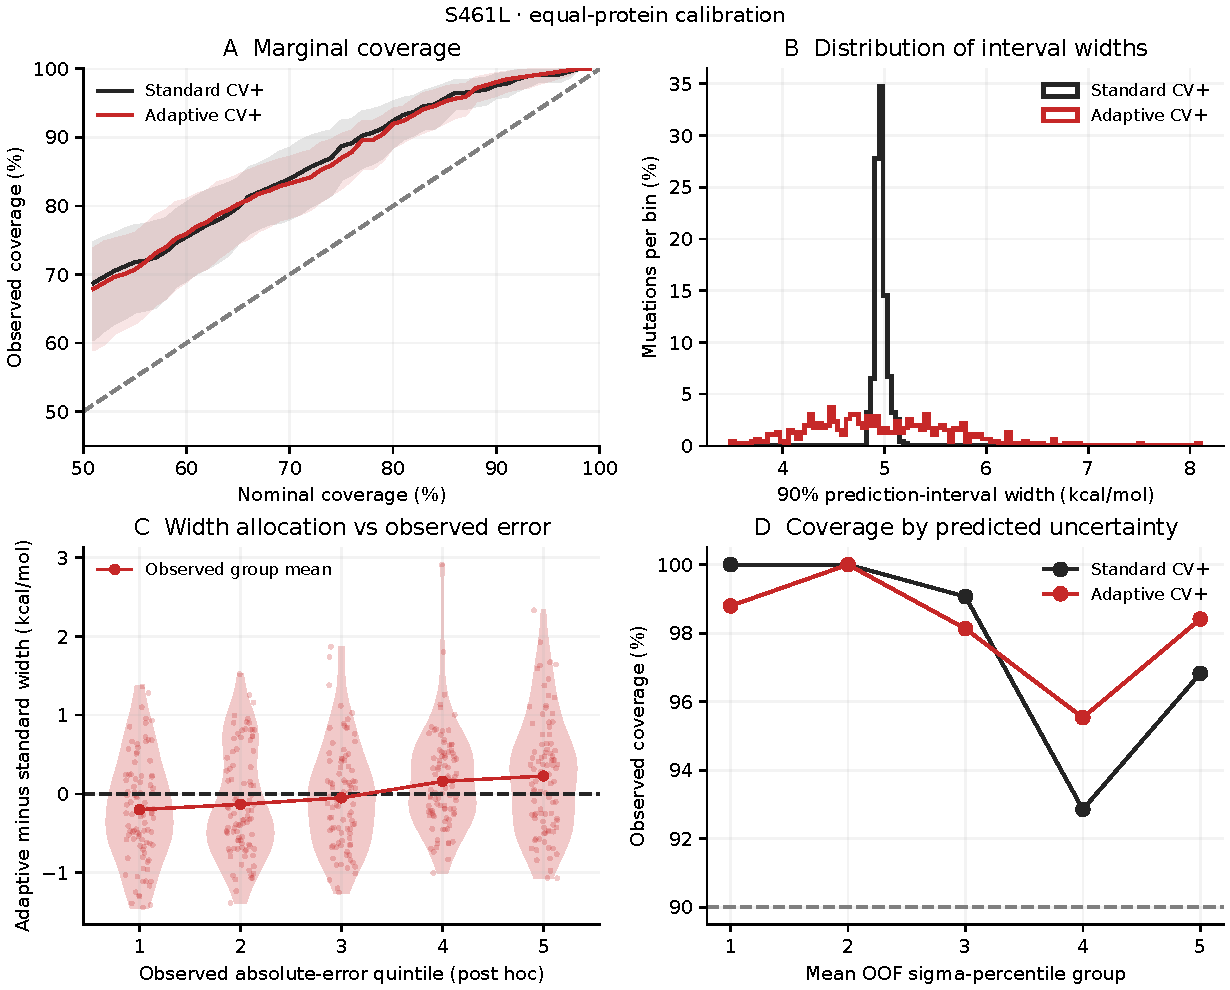
\includegraphics[width=0.96\textwidth]{s461l_uncertainty.pdf}
\caption{S461L counterpart of Fig.~\ref{fig:uncertainty}, using median predictions and
protein-weighted calibration. Panels and bootstrap procedure are identical. S461L overlaps
with S669L and is not an independent replication.}
\label{fig:s461}
\end{figure}
\clearpage

\begin{figure}[!ht]
\centering
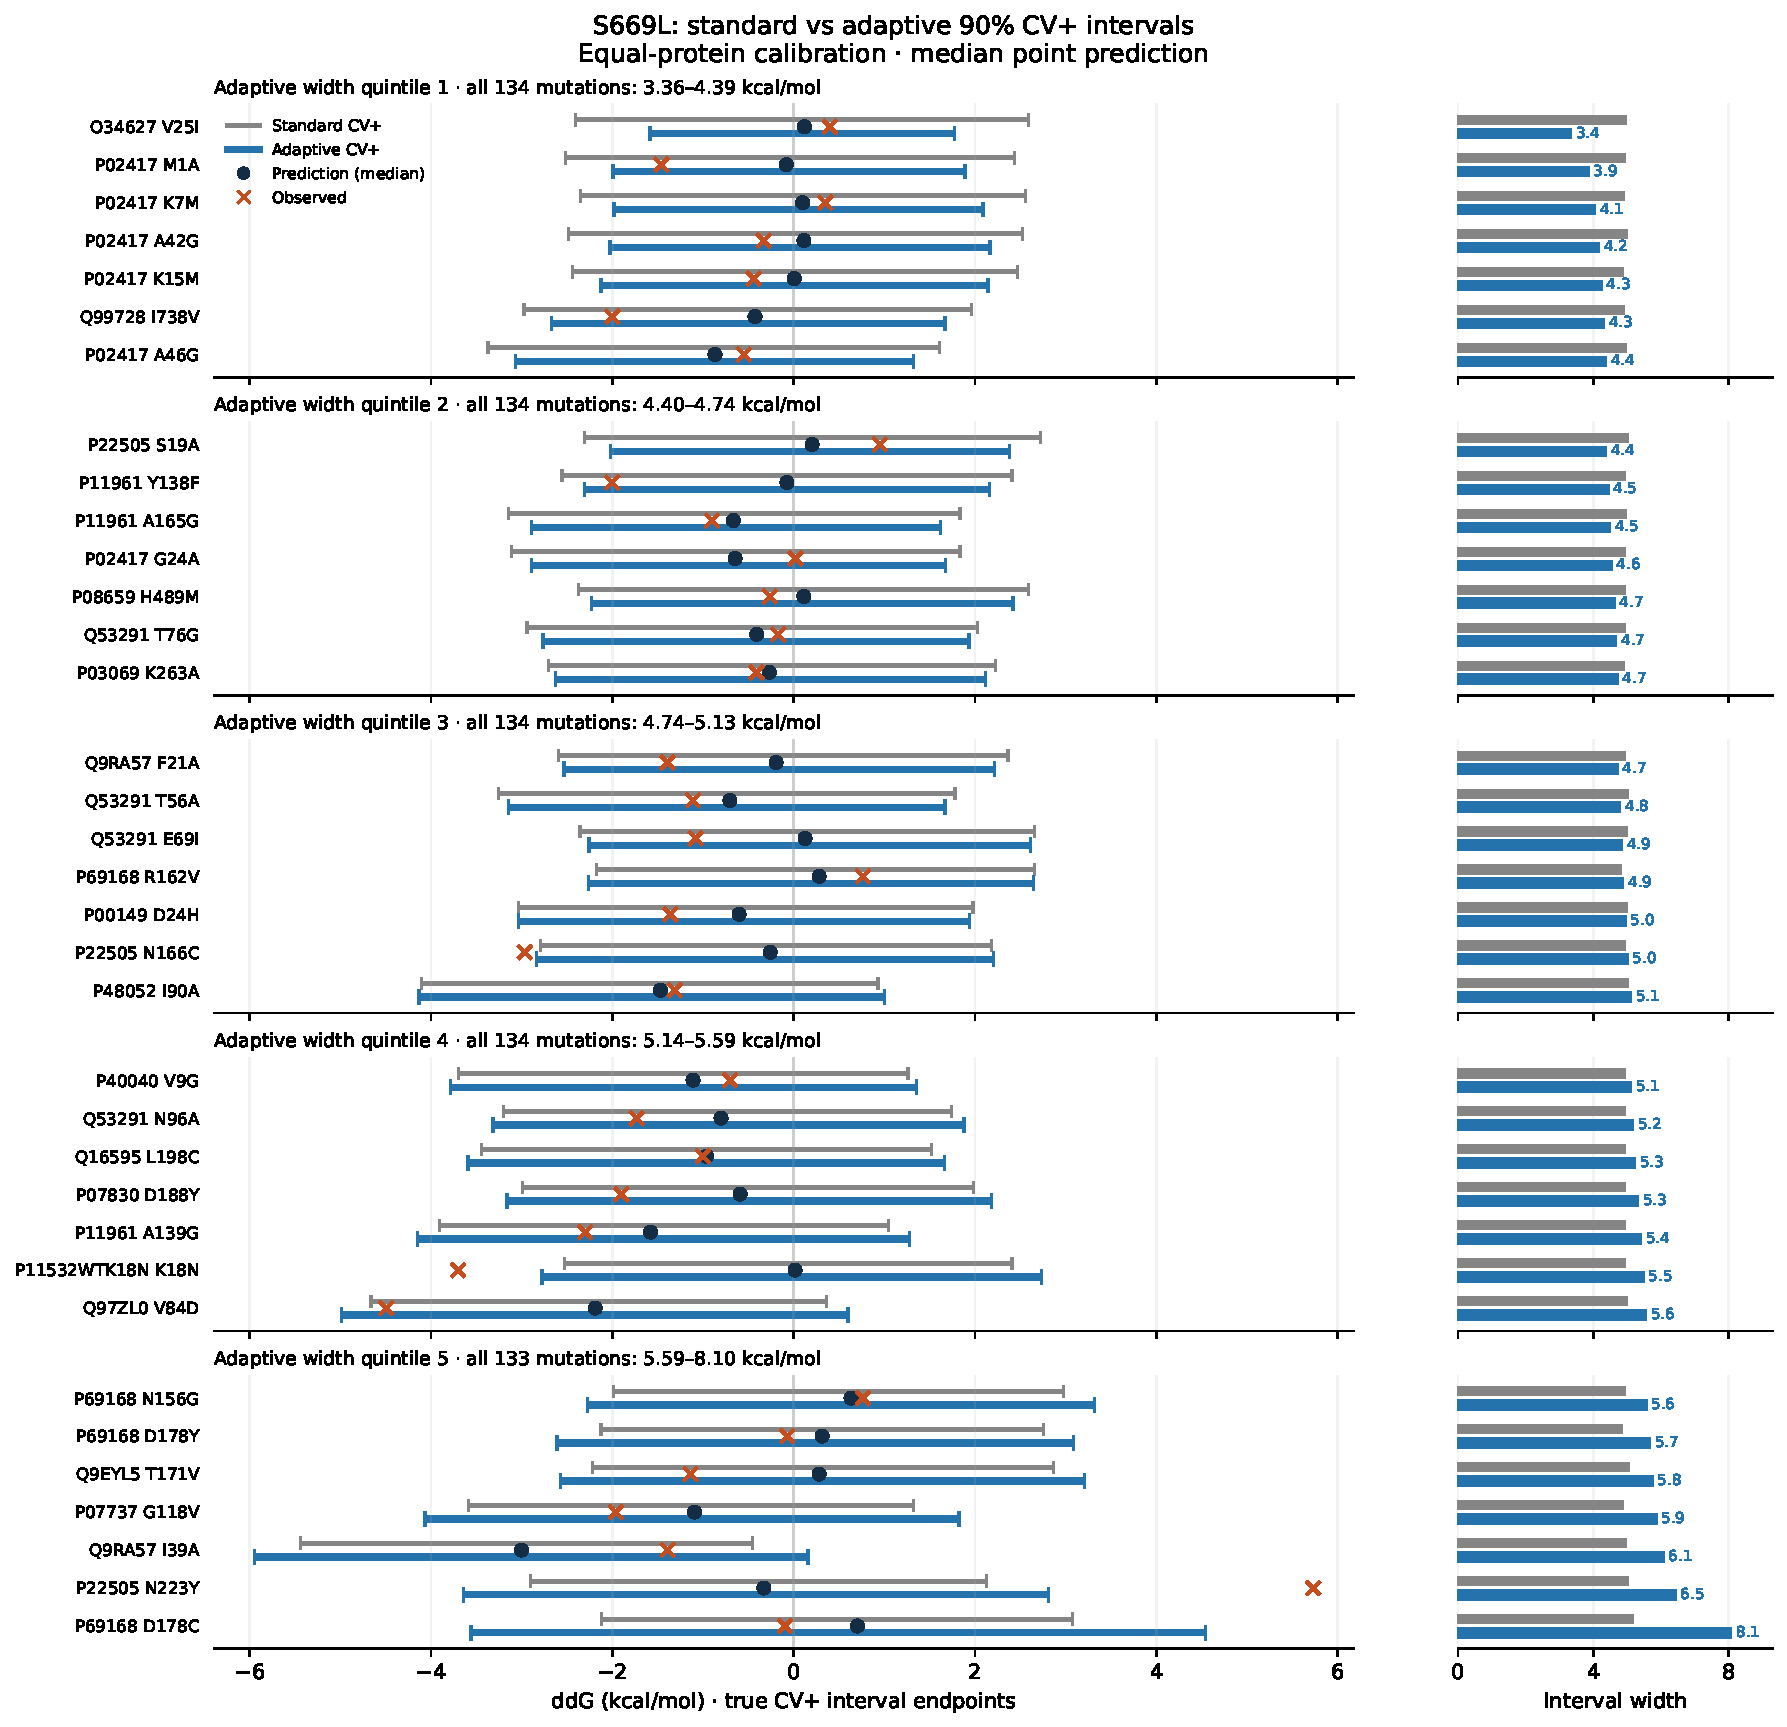
\includegraphics[width=0.93\textwidth,height=0.81\textheight,keepaspectratio]{s669l_interval_examples.pdf}
\caption{Width-stratified S669L examples with standard and adaptive protein-weighted 90\%
intervals and shared median predictions. Seven mutations are selected at evenly spaced width
ranks within each of five adaptive-width quintiles, including each group's endpoints.
Selection uses interval width only, without target error or coverage. Gray and blue lines
show actual standard and adaptive endpoints, slightly offset vertically for visibility;
side bars compare their widths. The 35 examples are illustrative, not a separate test set.}
\label{fig:examples}
\end{figure}
\clearpage

\begin{figure}[!ht]
\centering
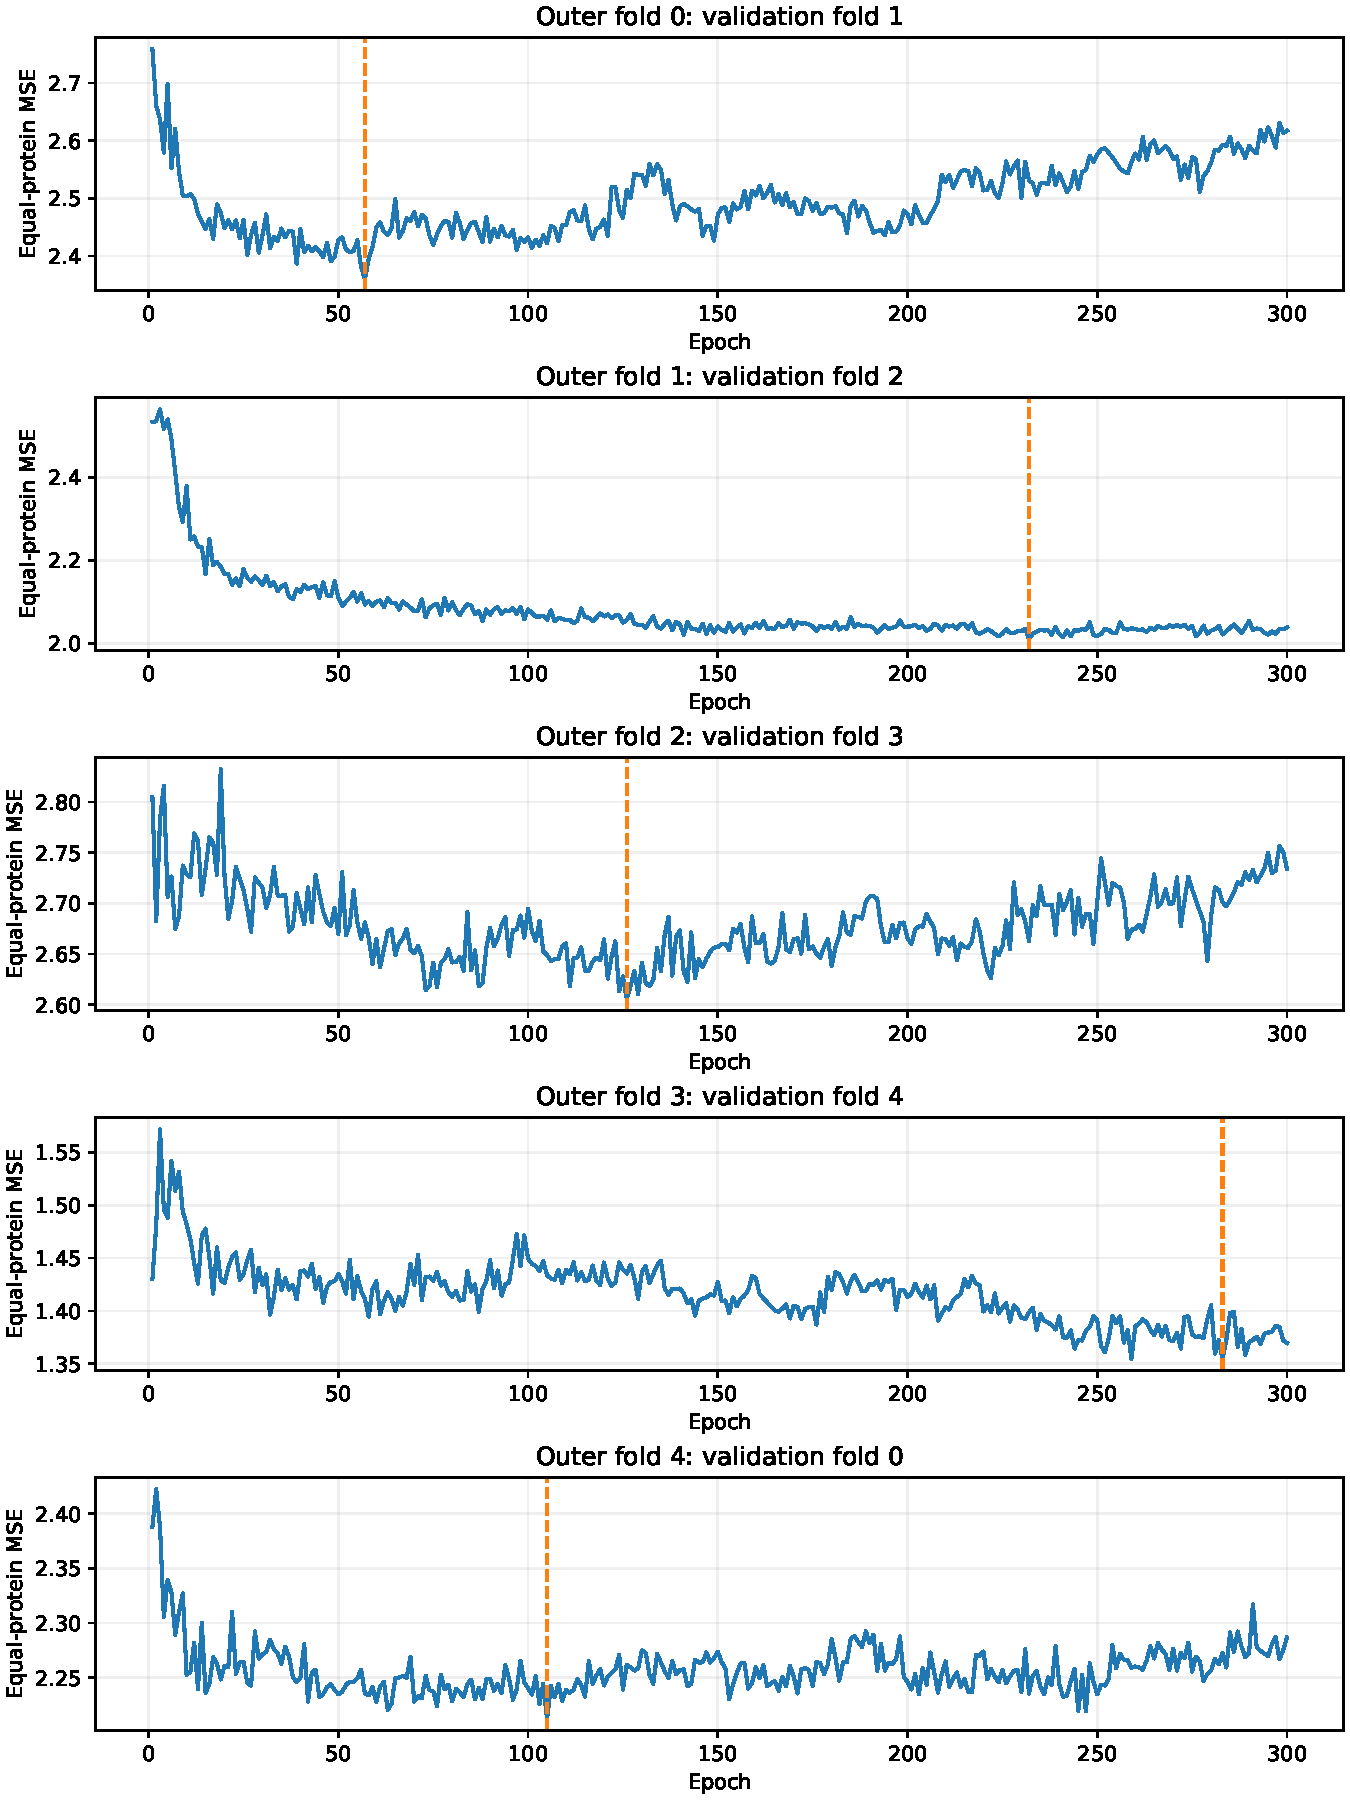
\includegraphics[width=0.82\textwidth,height=0.81\textheight,keepaspectratio]{epoch_selection.pdf}
\caption{Protein-averaged MSE on the five internal validation folds over 300 epochs.
Dashed lines mark the selected epochs 57, 232, 126, 283 and 105. Each curve comes from an
inner model trained on three folds and excludes the associated outer calibration fold.}
\label{fig:epochs}
\end{figure}
\clearpage



\clearpage

\twocolumn
\bibliographystyle{unsrtnat}
\bibliography{references}

\end{document}
